\chapter{\ifproject%
\ifenglish Project Structure and Methodology\else โครงสร้างและขั้นตอนการทำงาน\fi
\else%
\ifenglish Project Structure\else โครงสร้างของโครงงาน\fi
\fi
}

\makeatletter

% \renewcommand\section{\@startsection {section}{1}{\z@}%
%                                    {13.5ex \@plus -1ex \@minus -.2ex}%
%                                    {2.3ex \@plus.2ex}%
%                                    {\normalfont\large\bfseries}}

\makeatother
%\vspace{2ex}
% \titleformat{\section}{\normalfont\bfseries}{\thesection}{1em}{}
% \titlespacing*{\section}{0pt}{10ex}{0pt}

\section{โครงสร้างของระบบ}
\subsection{หน้าเว็บสำหรับนักศึกษา}
\begin{center}
สำหรับนักศึกษา จะต้องล็อคอินผ่าน CMU Account ของมหาวิทยาลัยเพื่อที่จะสามารถเข้าสู่ระบบได้
\end{center}

\begin{figure}[H]
  \begin{center}
    \subfigure{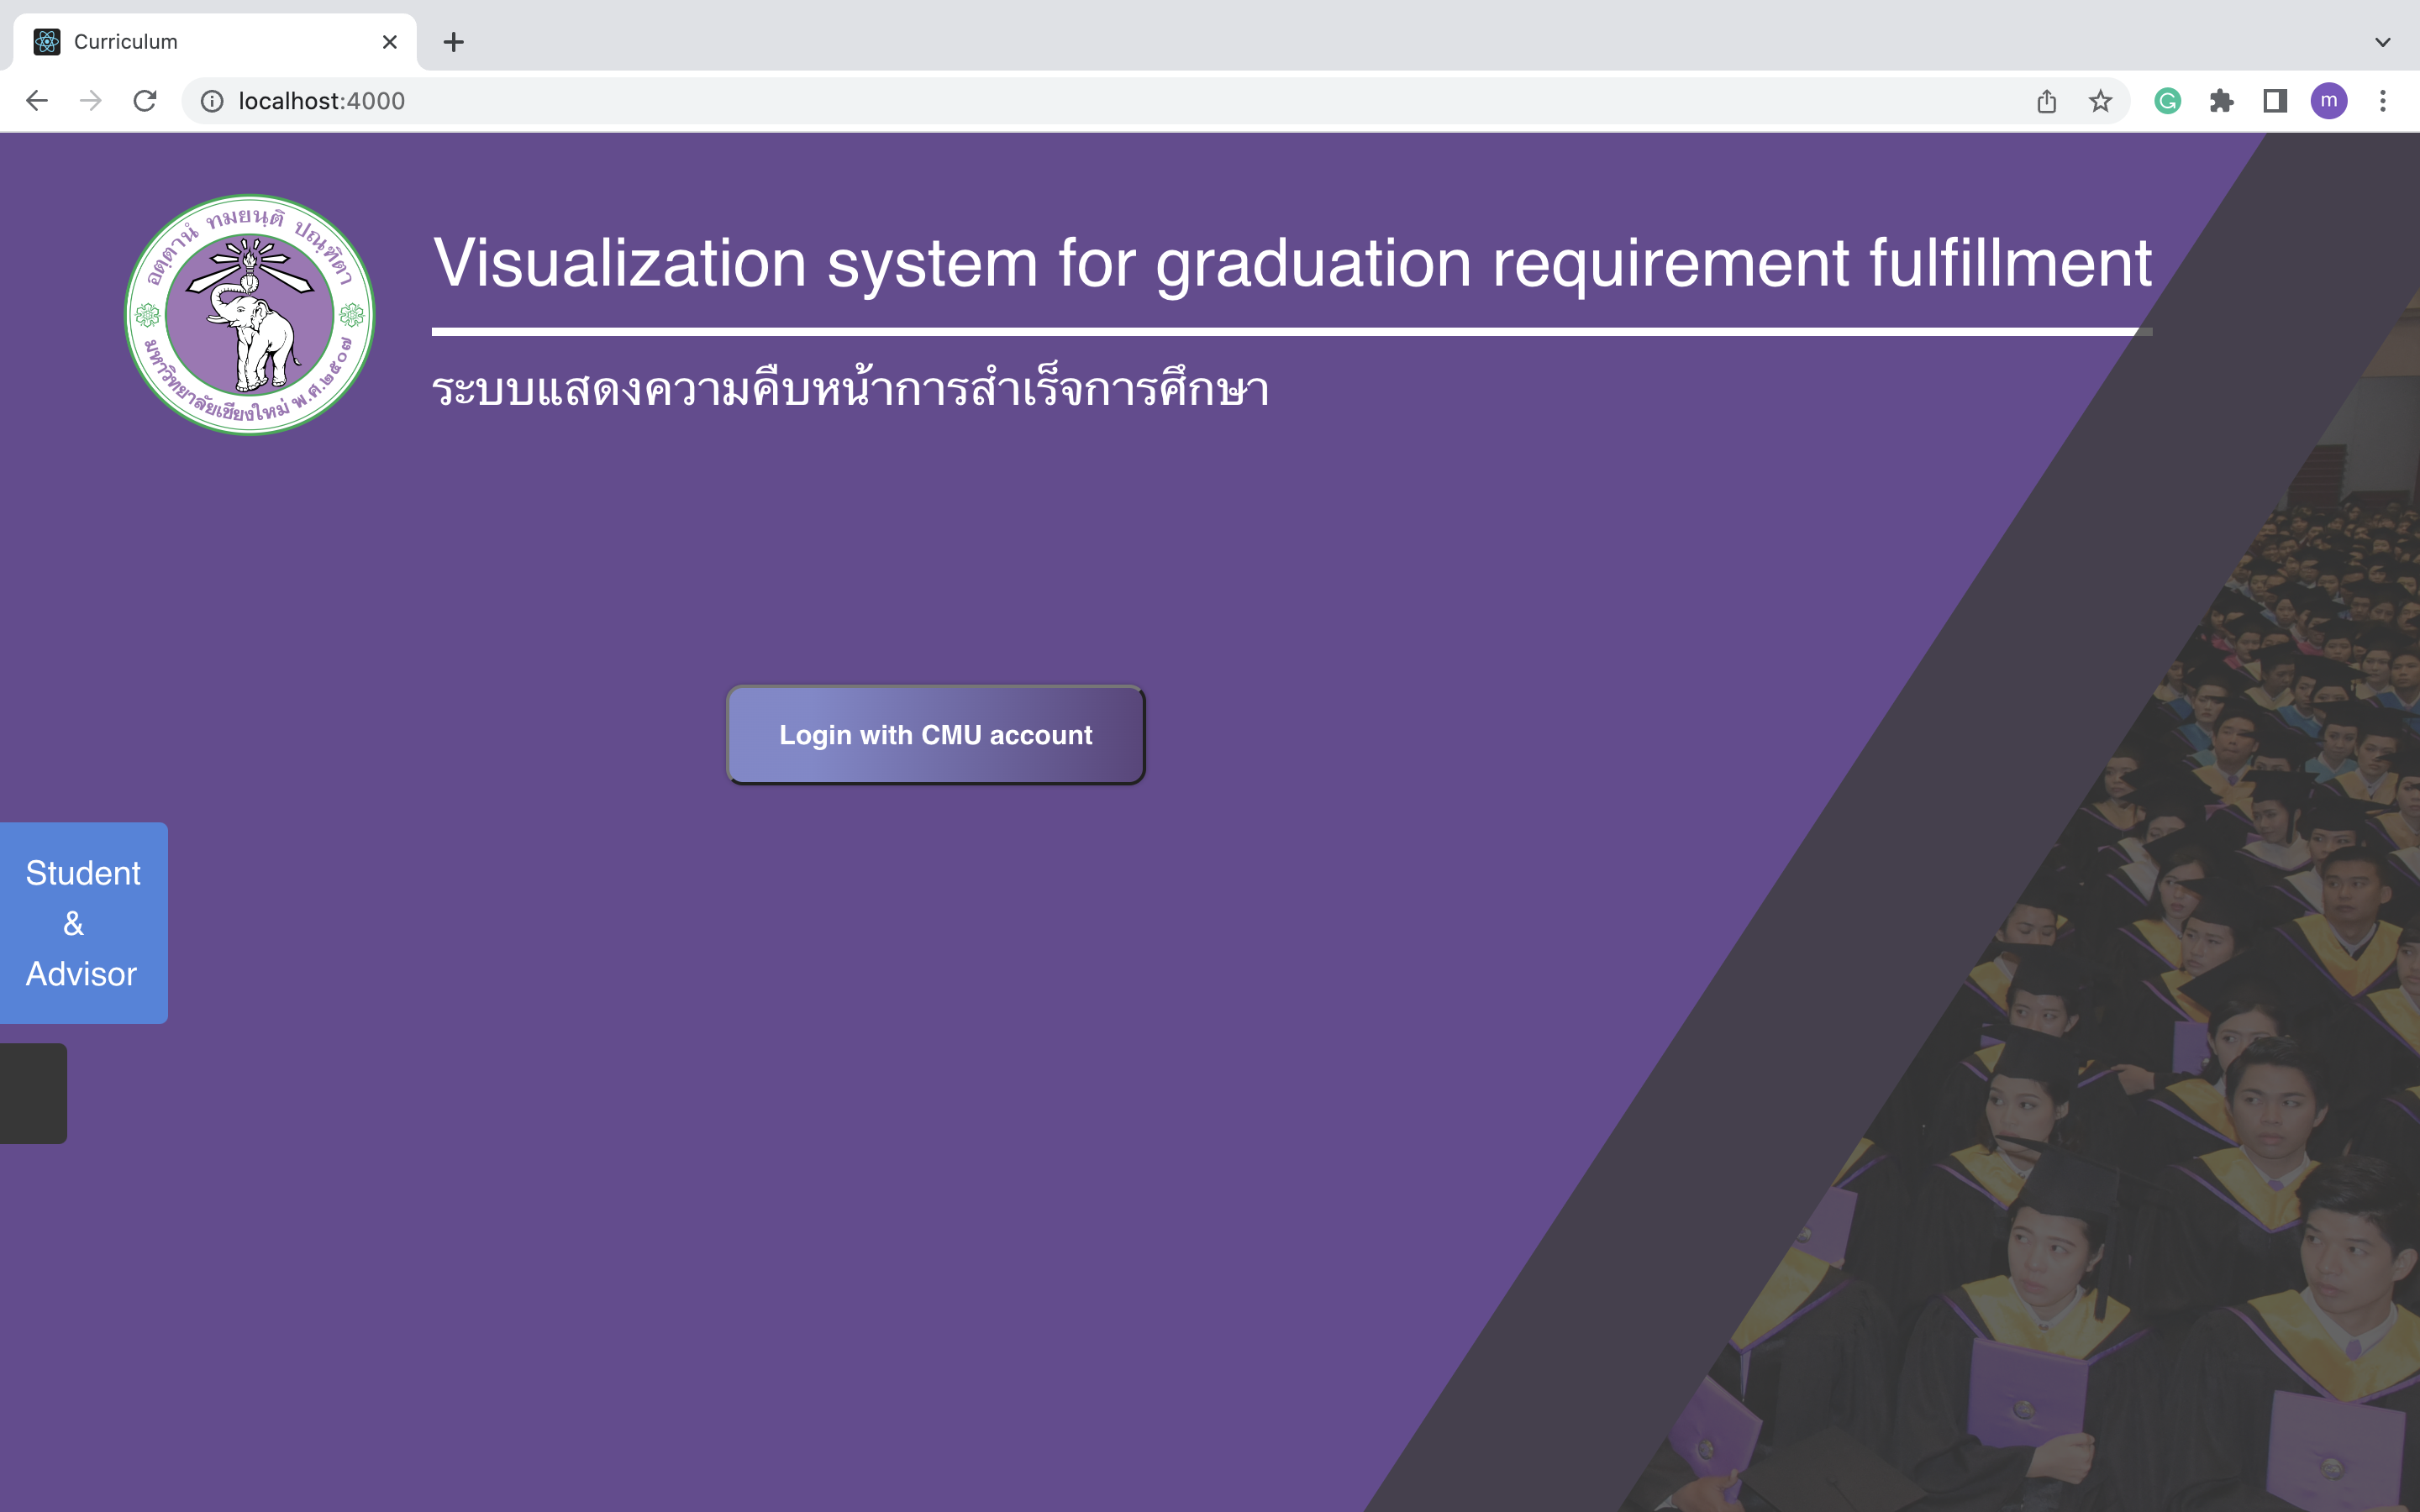
\includegraphics[width=0.8\textwidth]{login.png}}
    \subfigure{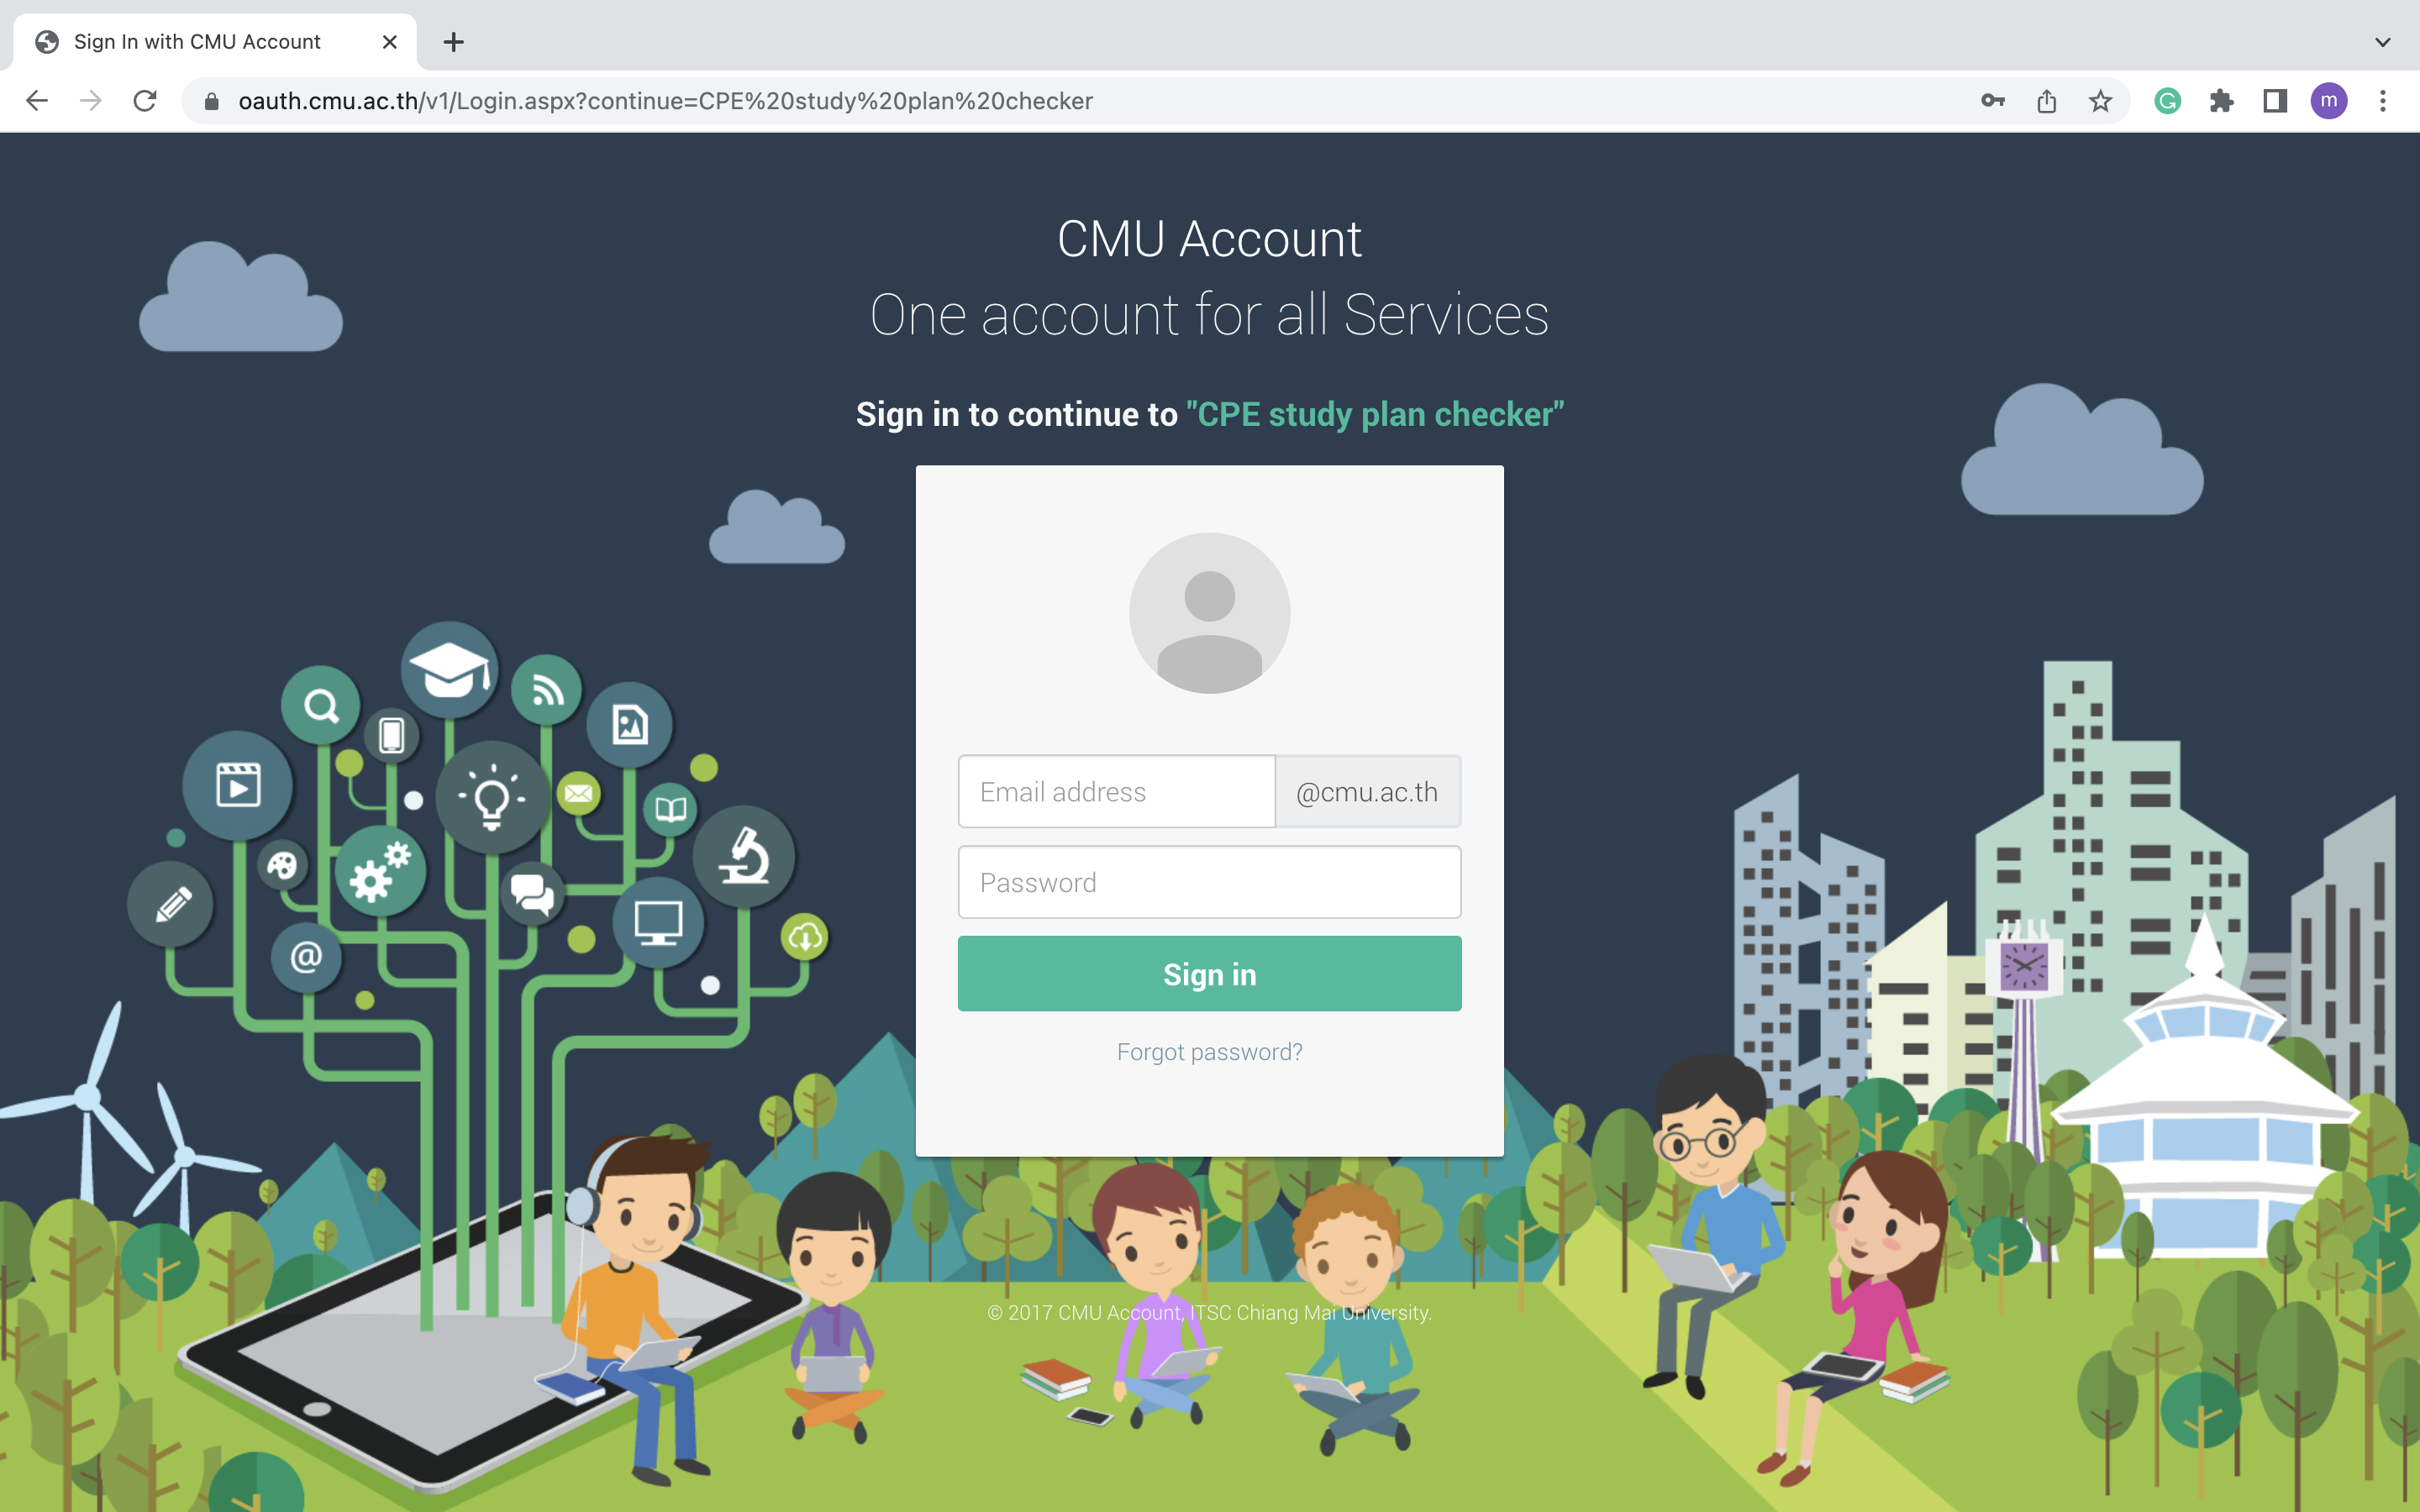
\includegraphics[width=0.8\textwidth]{oauth.png}}
  \end{center}
  \caption{หน้า Student Login}
  \label{fig:login}
\end{figure}

% \begin{center}
%   ตัวเลือกแผนการเรียน
% \end{center}

\begin{figure}[H]
  \begin{center}
    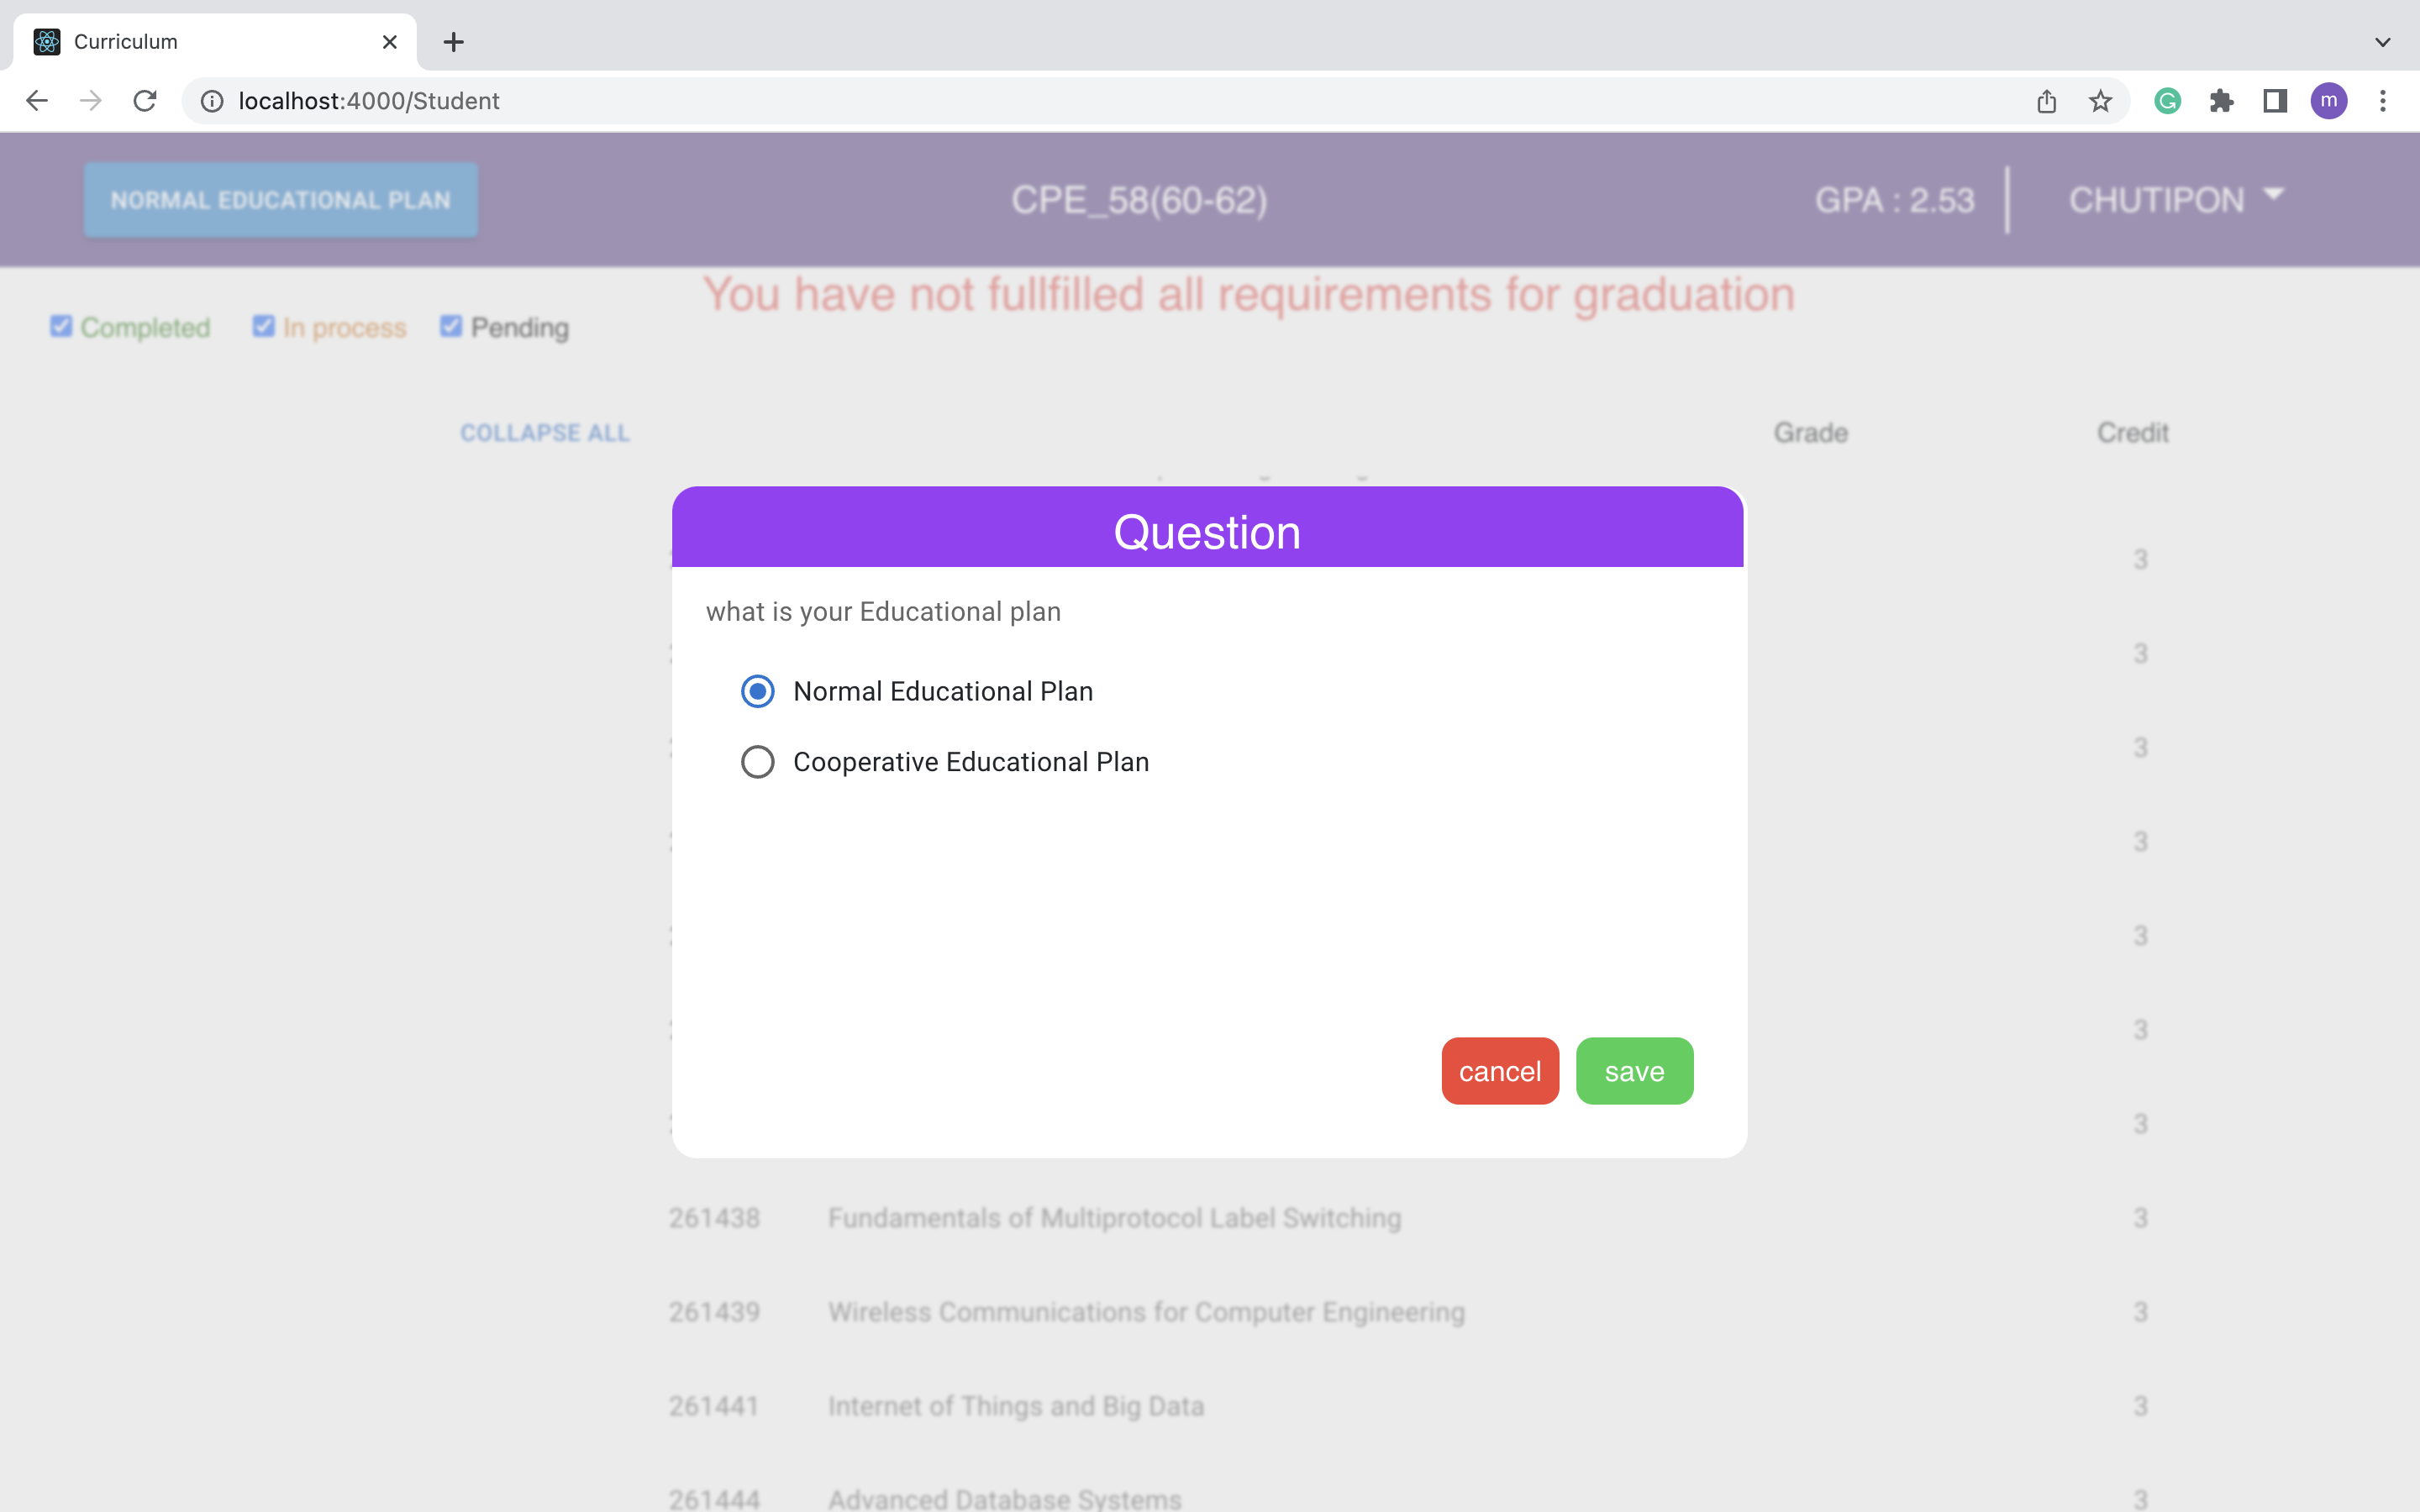
\includegraphics[width=0.8\textwidth]{question.png}
    \caption{หน้าเลือกเเผนการศึกษา}
    \label{fig:question}
  \end{center}
\end{figure}

\begin{figure}[H]
  \begin{center}
    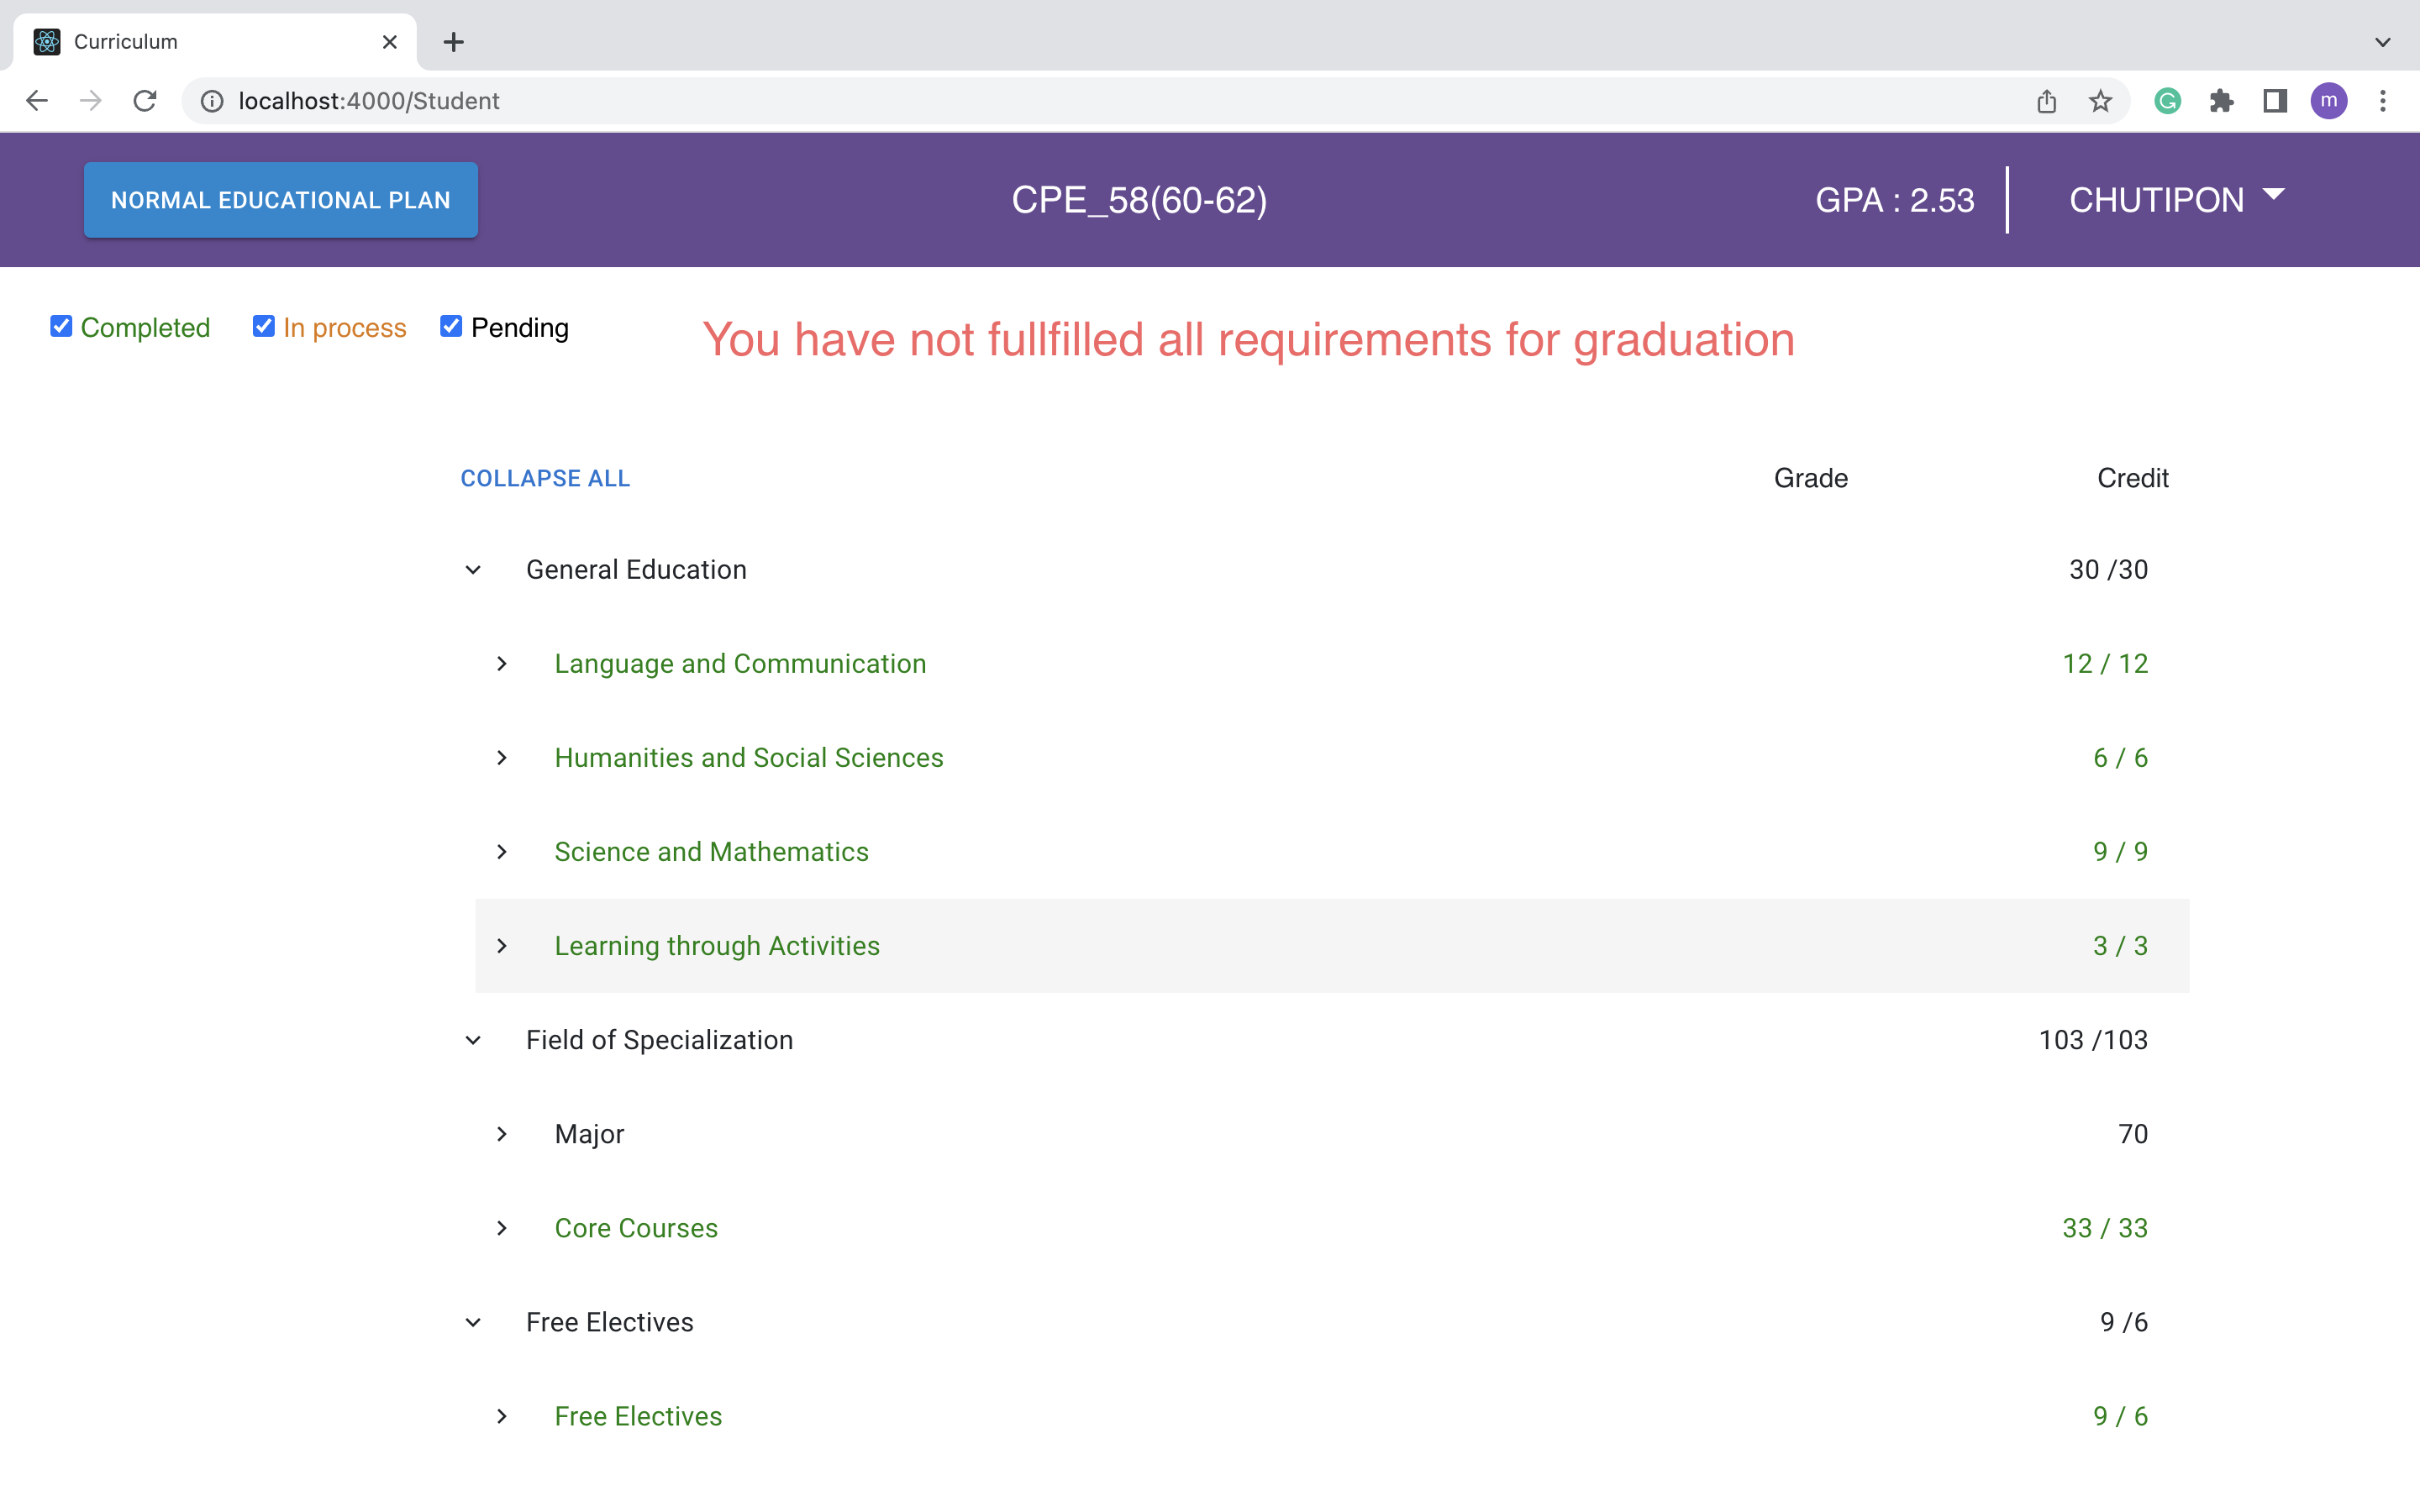
\includegraphics[width=0.8\textwidth]{student.png}
    \caption{หน้าเเสดงผลการศึกษา}
    \label{fig:student}
  \end{center}
\end{figure}

การใช้งานของนักศึกษา เมื่อเข้าสู่ระบบเป็นที่เรียบร้อยแล้วนั้น นักศึกษาจะเห็นโครงสร้างหลักสูตรของตนเองที่จะอธิบาย
รายวิชาในหมวดต่างๆ ได้แก่รายวิชาที่เรียนสำเร็จแล้ว (สถานะสีเขียวพร้อมเกรดที่ได้รับ) รายวิชาที่กำลังลงเรียนอยู่ในเทอมนั้น
(สถานะสีนํ้าตาล) และรายวิชาที่ยังไม่ได้ลงทะเบียนเรียนหรือเป็นวิชาที่ไม่ผ่านจากเทอมที่ผ่านมาและไม่ได้ลงเรียนอยู่ในเทอมนั้น (สถานะ
เเดง เเละเทา) ซึ่งนักศึกษาสามารถเลือกดูเพียงสถานะที่ตนเองสนใจได้โดยการเลือกฟังก์ชันเช็คบล็อค เพื่อแสดงสถานะที่มุมบนซ้ายมือของเว็บ
เพจ นอกจากนี้นักศึกษาสามารถเลือกแผนการเรียนและความถนัดในสาขาวิชาชีพของตนเองตามที่หลักสูตรกำหนดไว้ โดยการเลือกที่
ฟังก์ชันคำถามแล้วตอบคำถามตามที่ตนเองสนใจ

% \begin{figure}[b]
%   \begin{center}
%     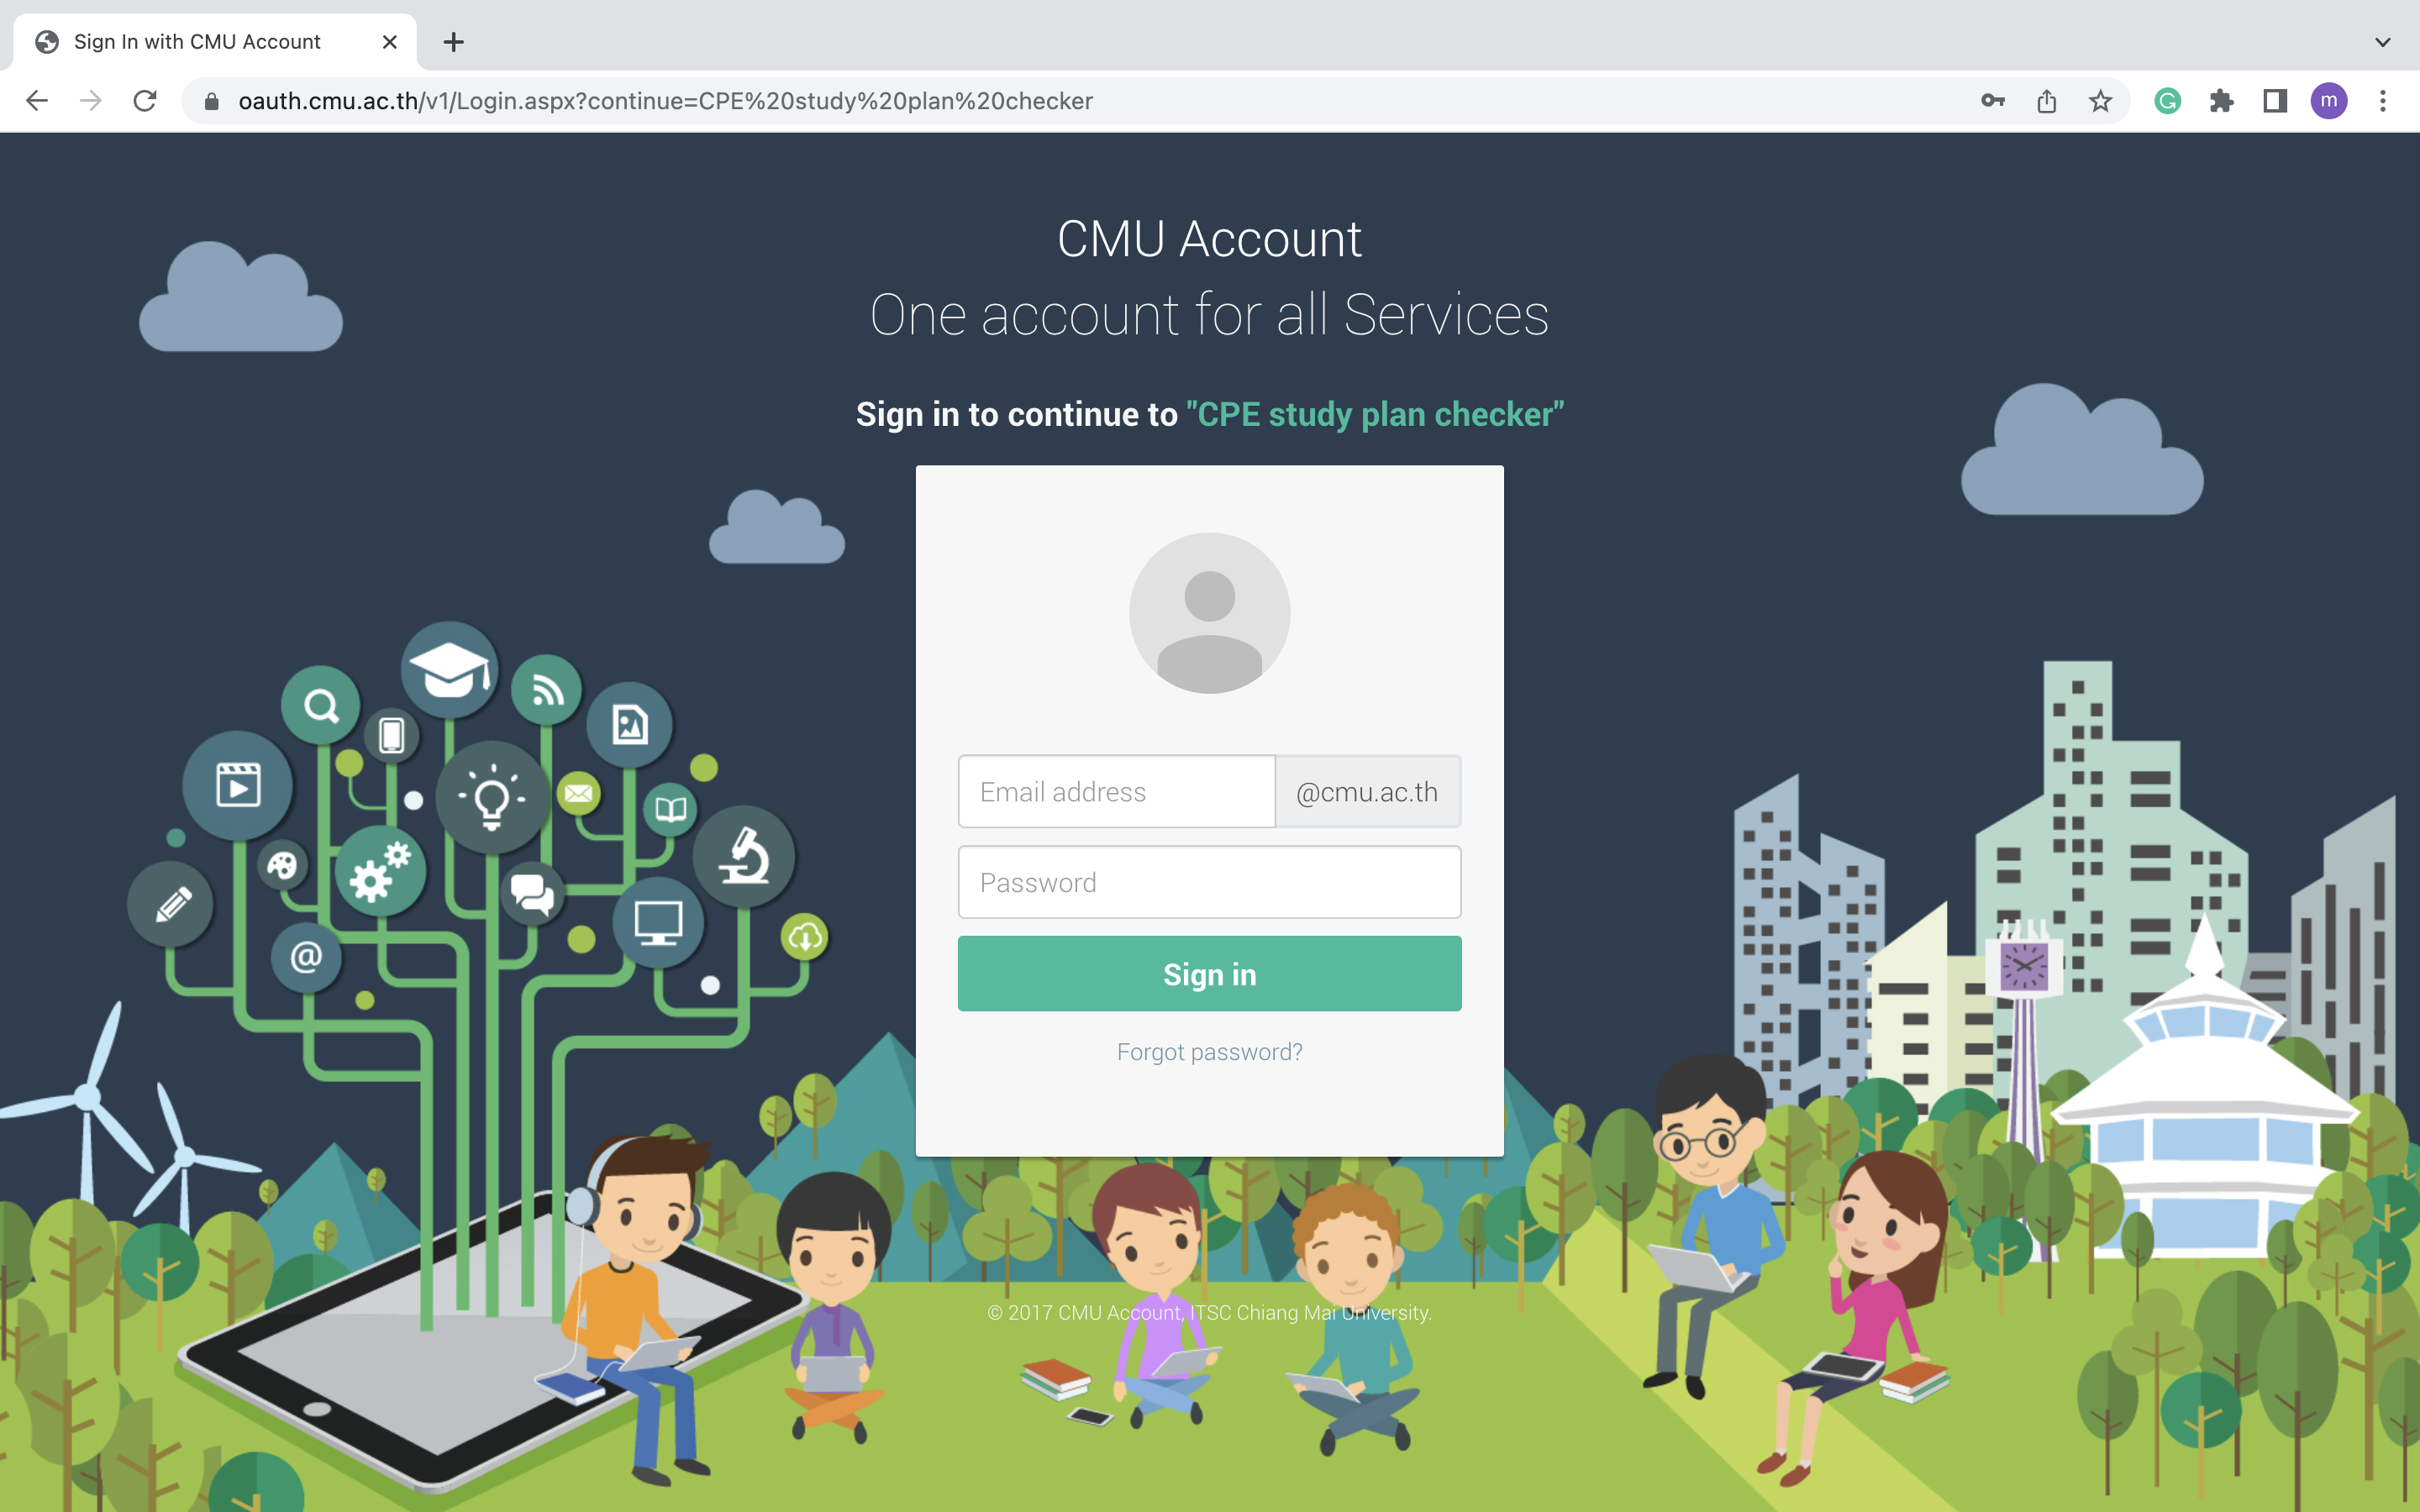
\includegraphics[width=0.8\textwidth]{oauth.png}
%     \caption{หน้า OAuth login}
%     \label{fig:oauth}
%   \end{center}
% \end{figure}

\subsection{หน้าเว็บสำหรับอาจารย์ที่ปรึกษา}

\begin{figure}[H]
  \begin{center}
    \subfigure{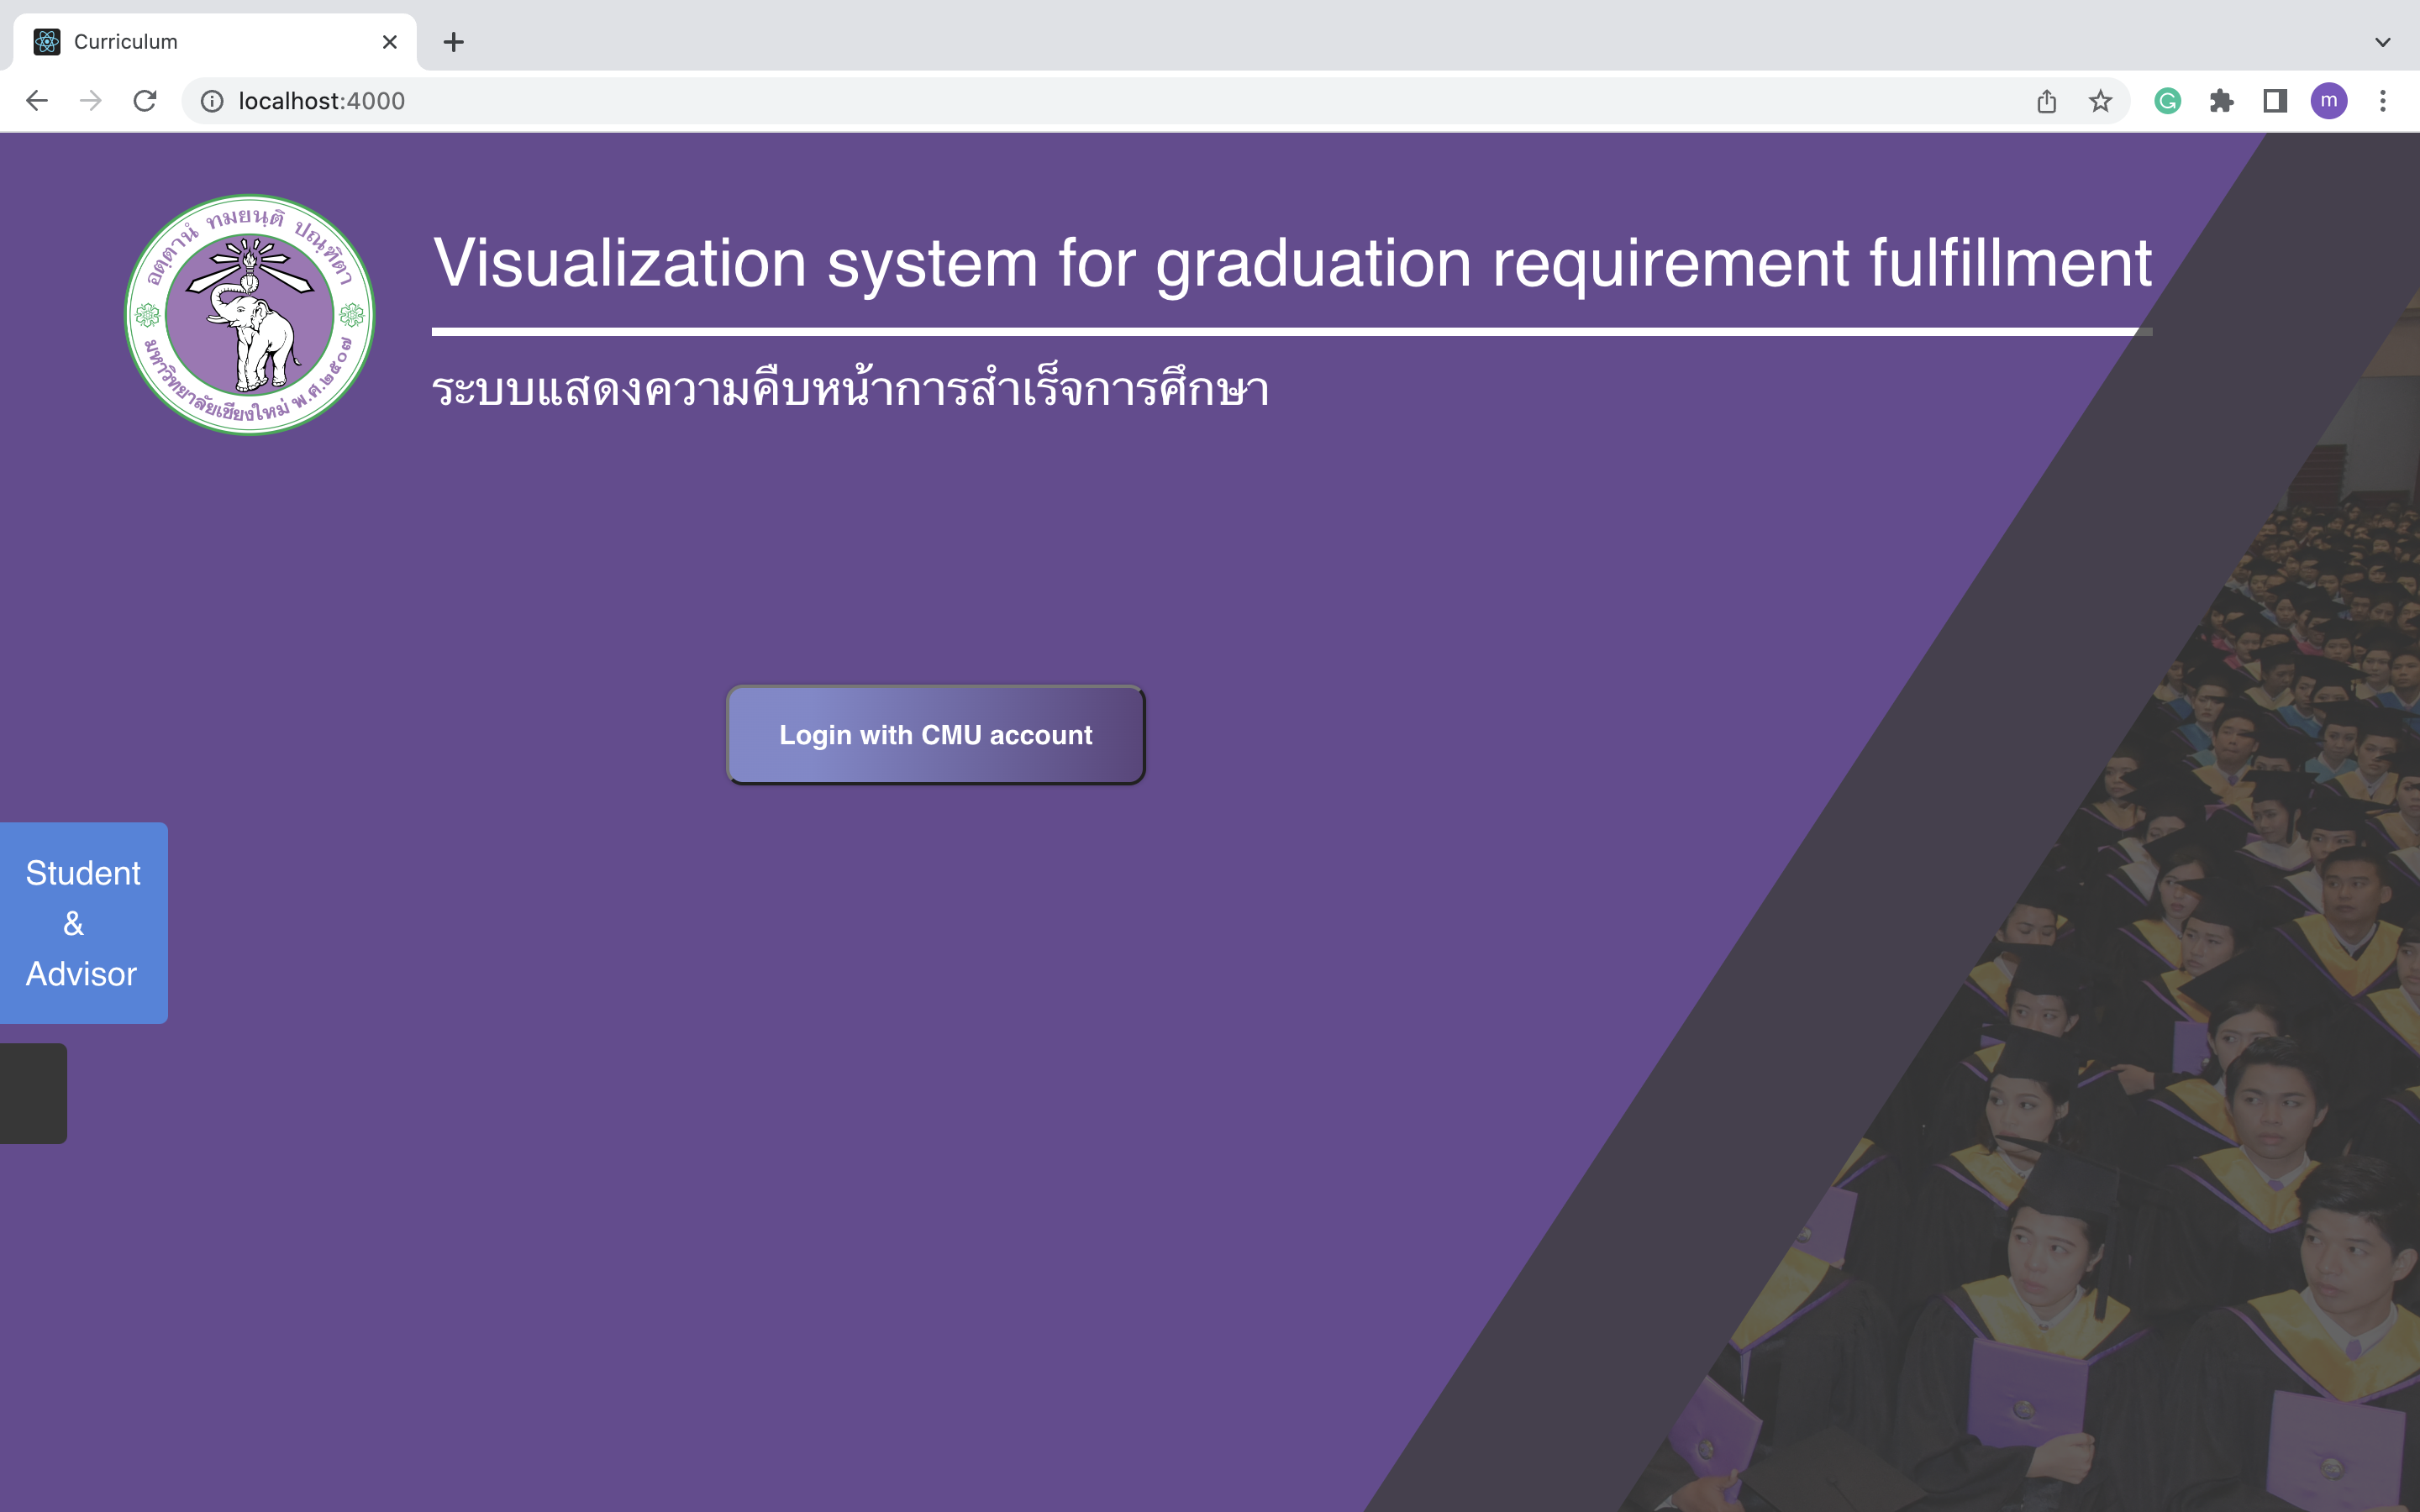
\includegraphics[width=0.8\textwidth]{login.png}}
    \subfigure{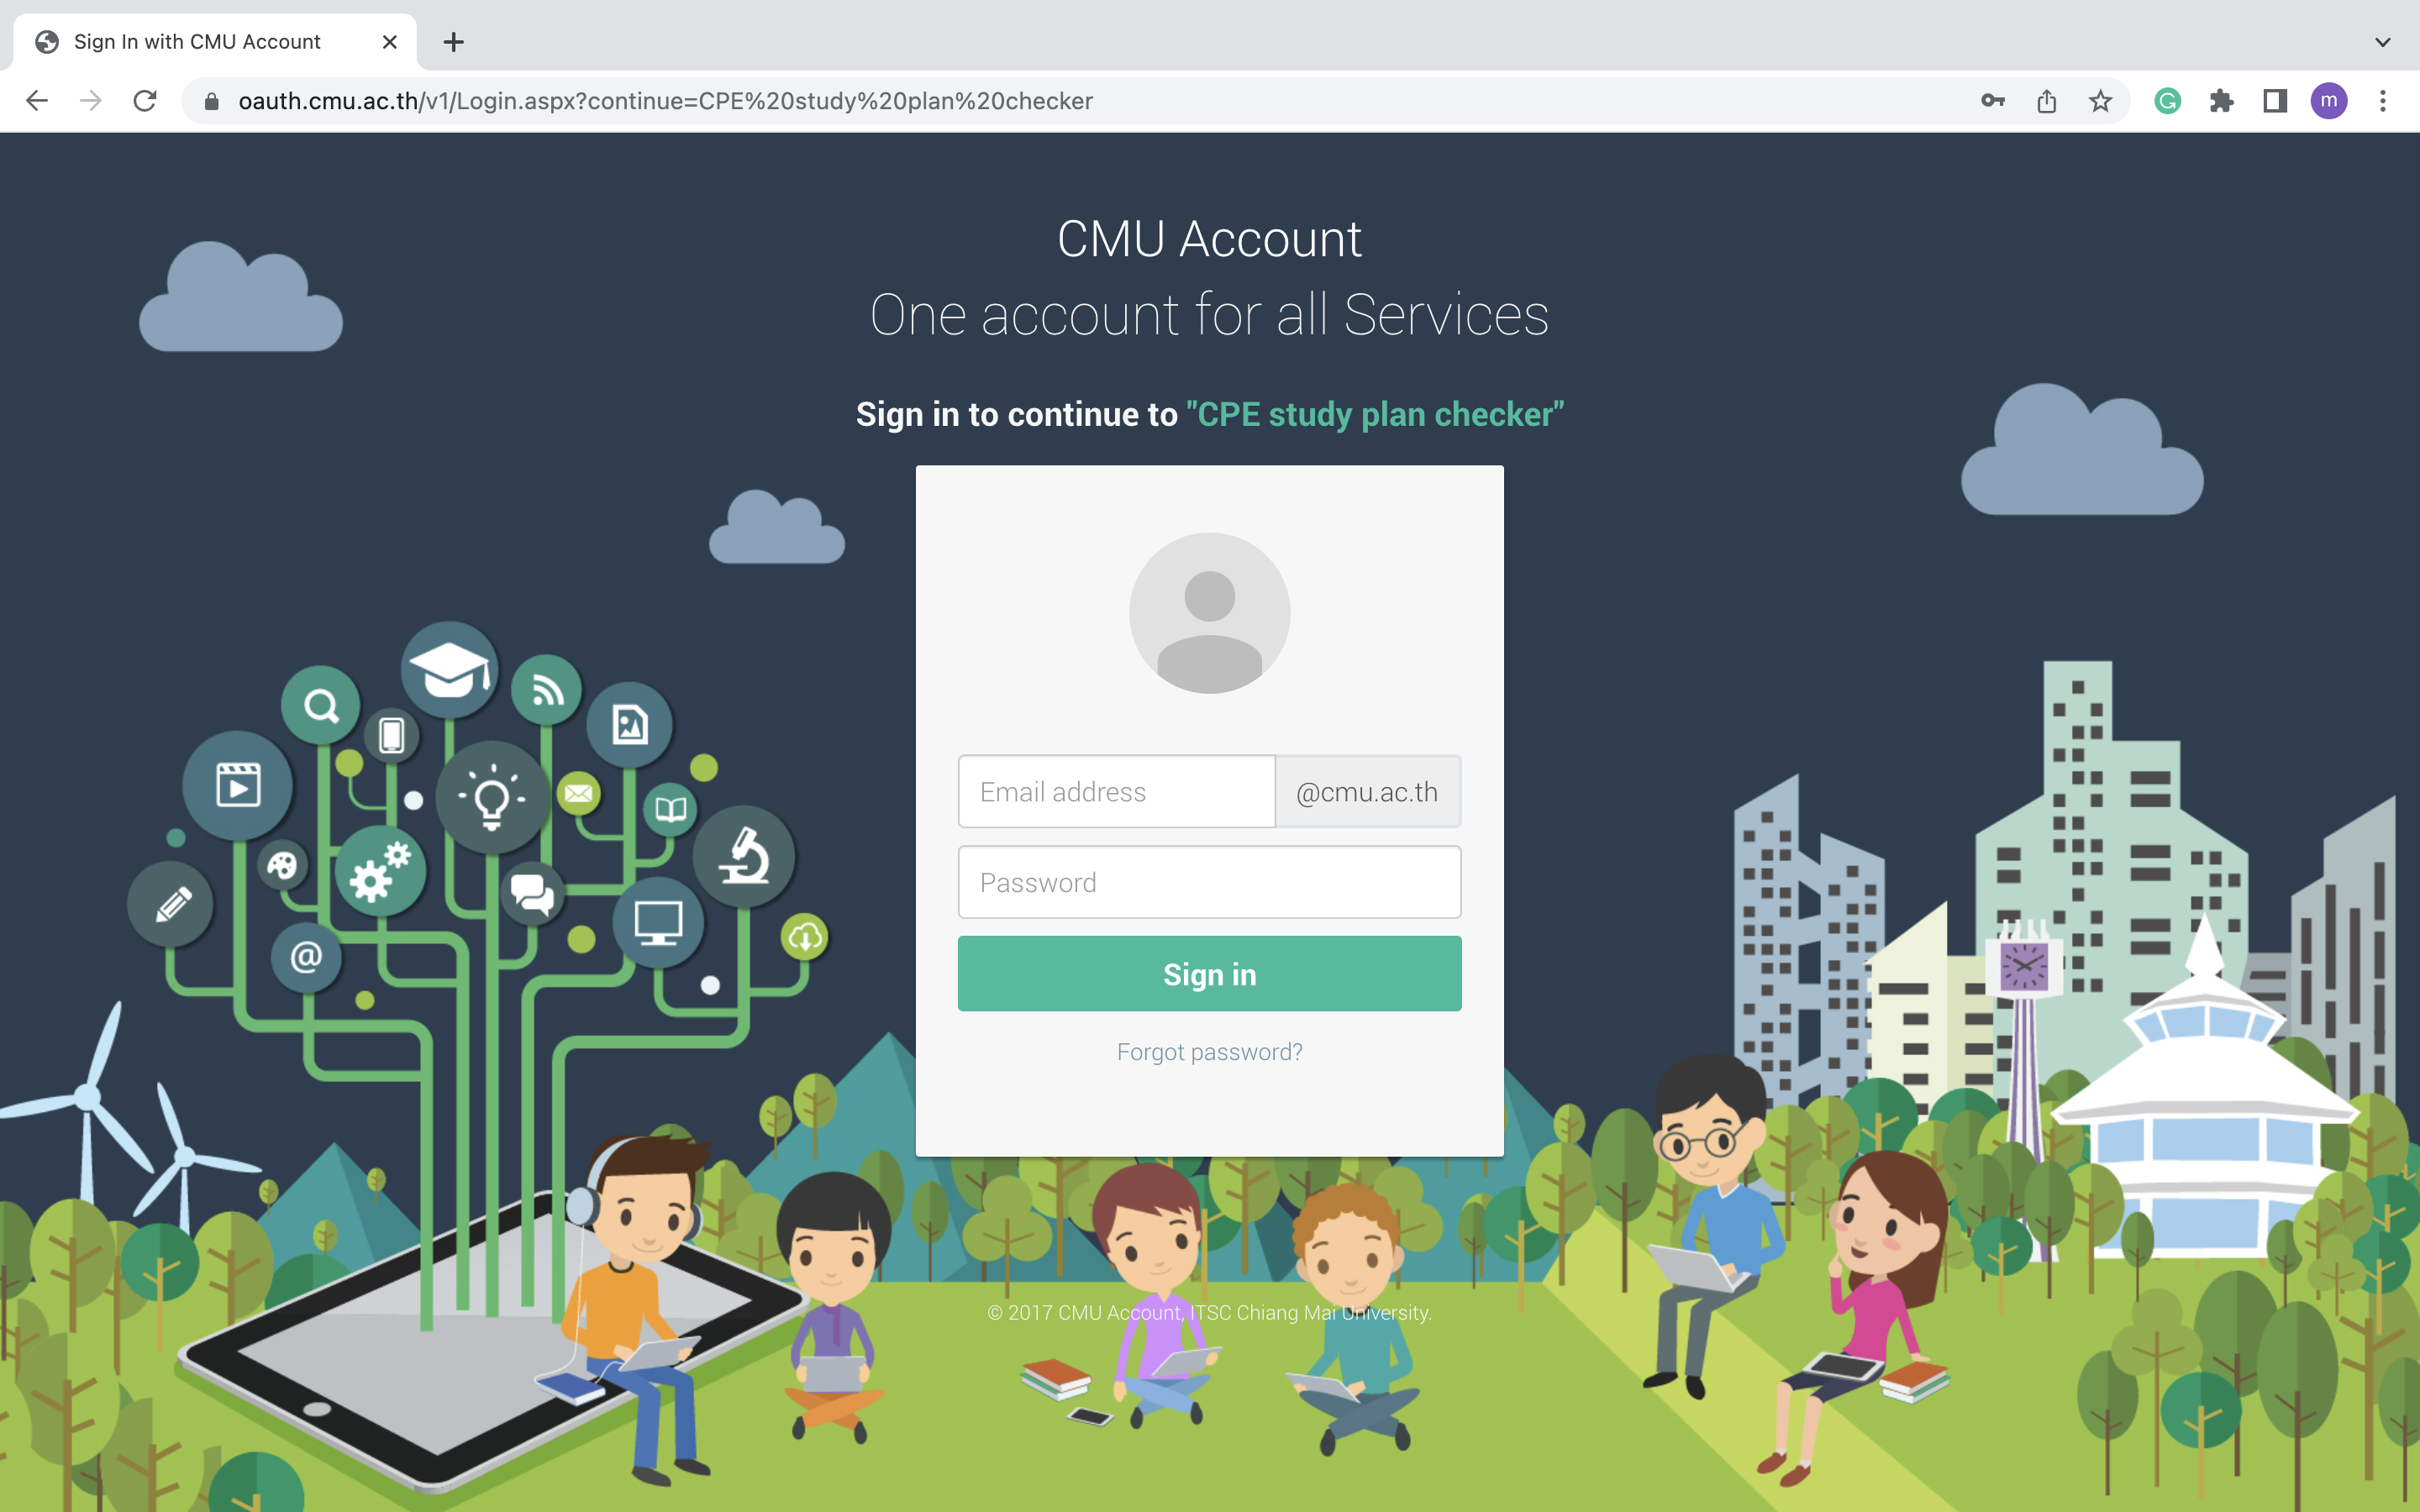
\includegraphics[width=0.8\textwidth]{oauth.png}}
  \end{center}
  \caption{หน้า Advisor Login}
  \label{fig:advisor_login}
\end{figure}

\begin{figure}[H]
  \begin{center}
    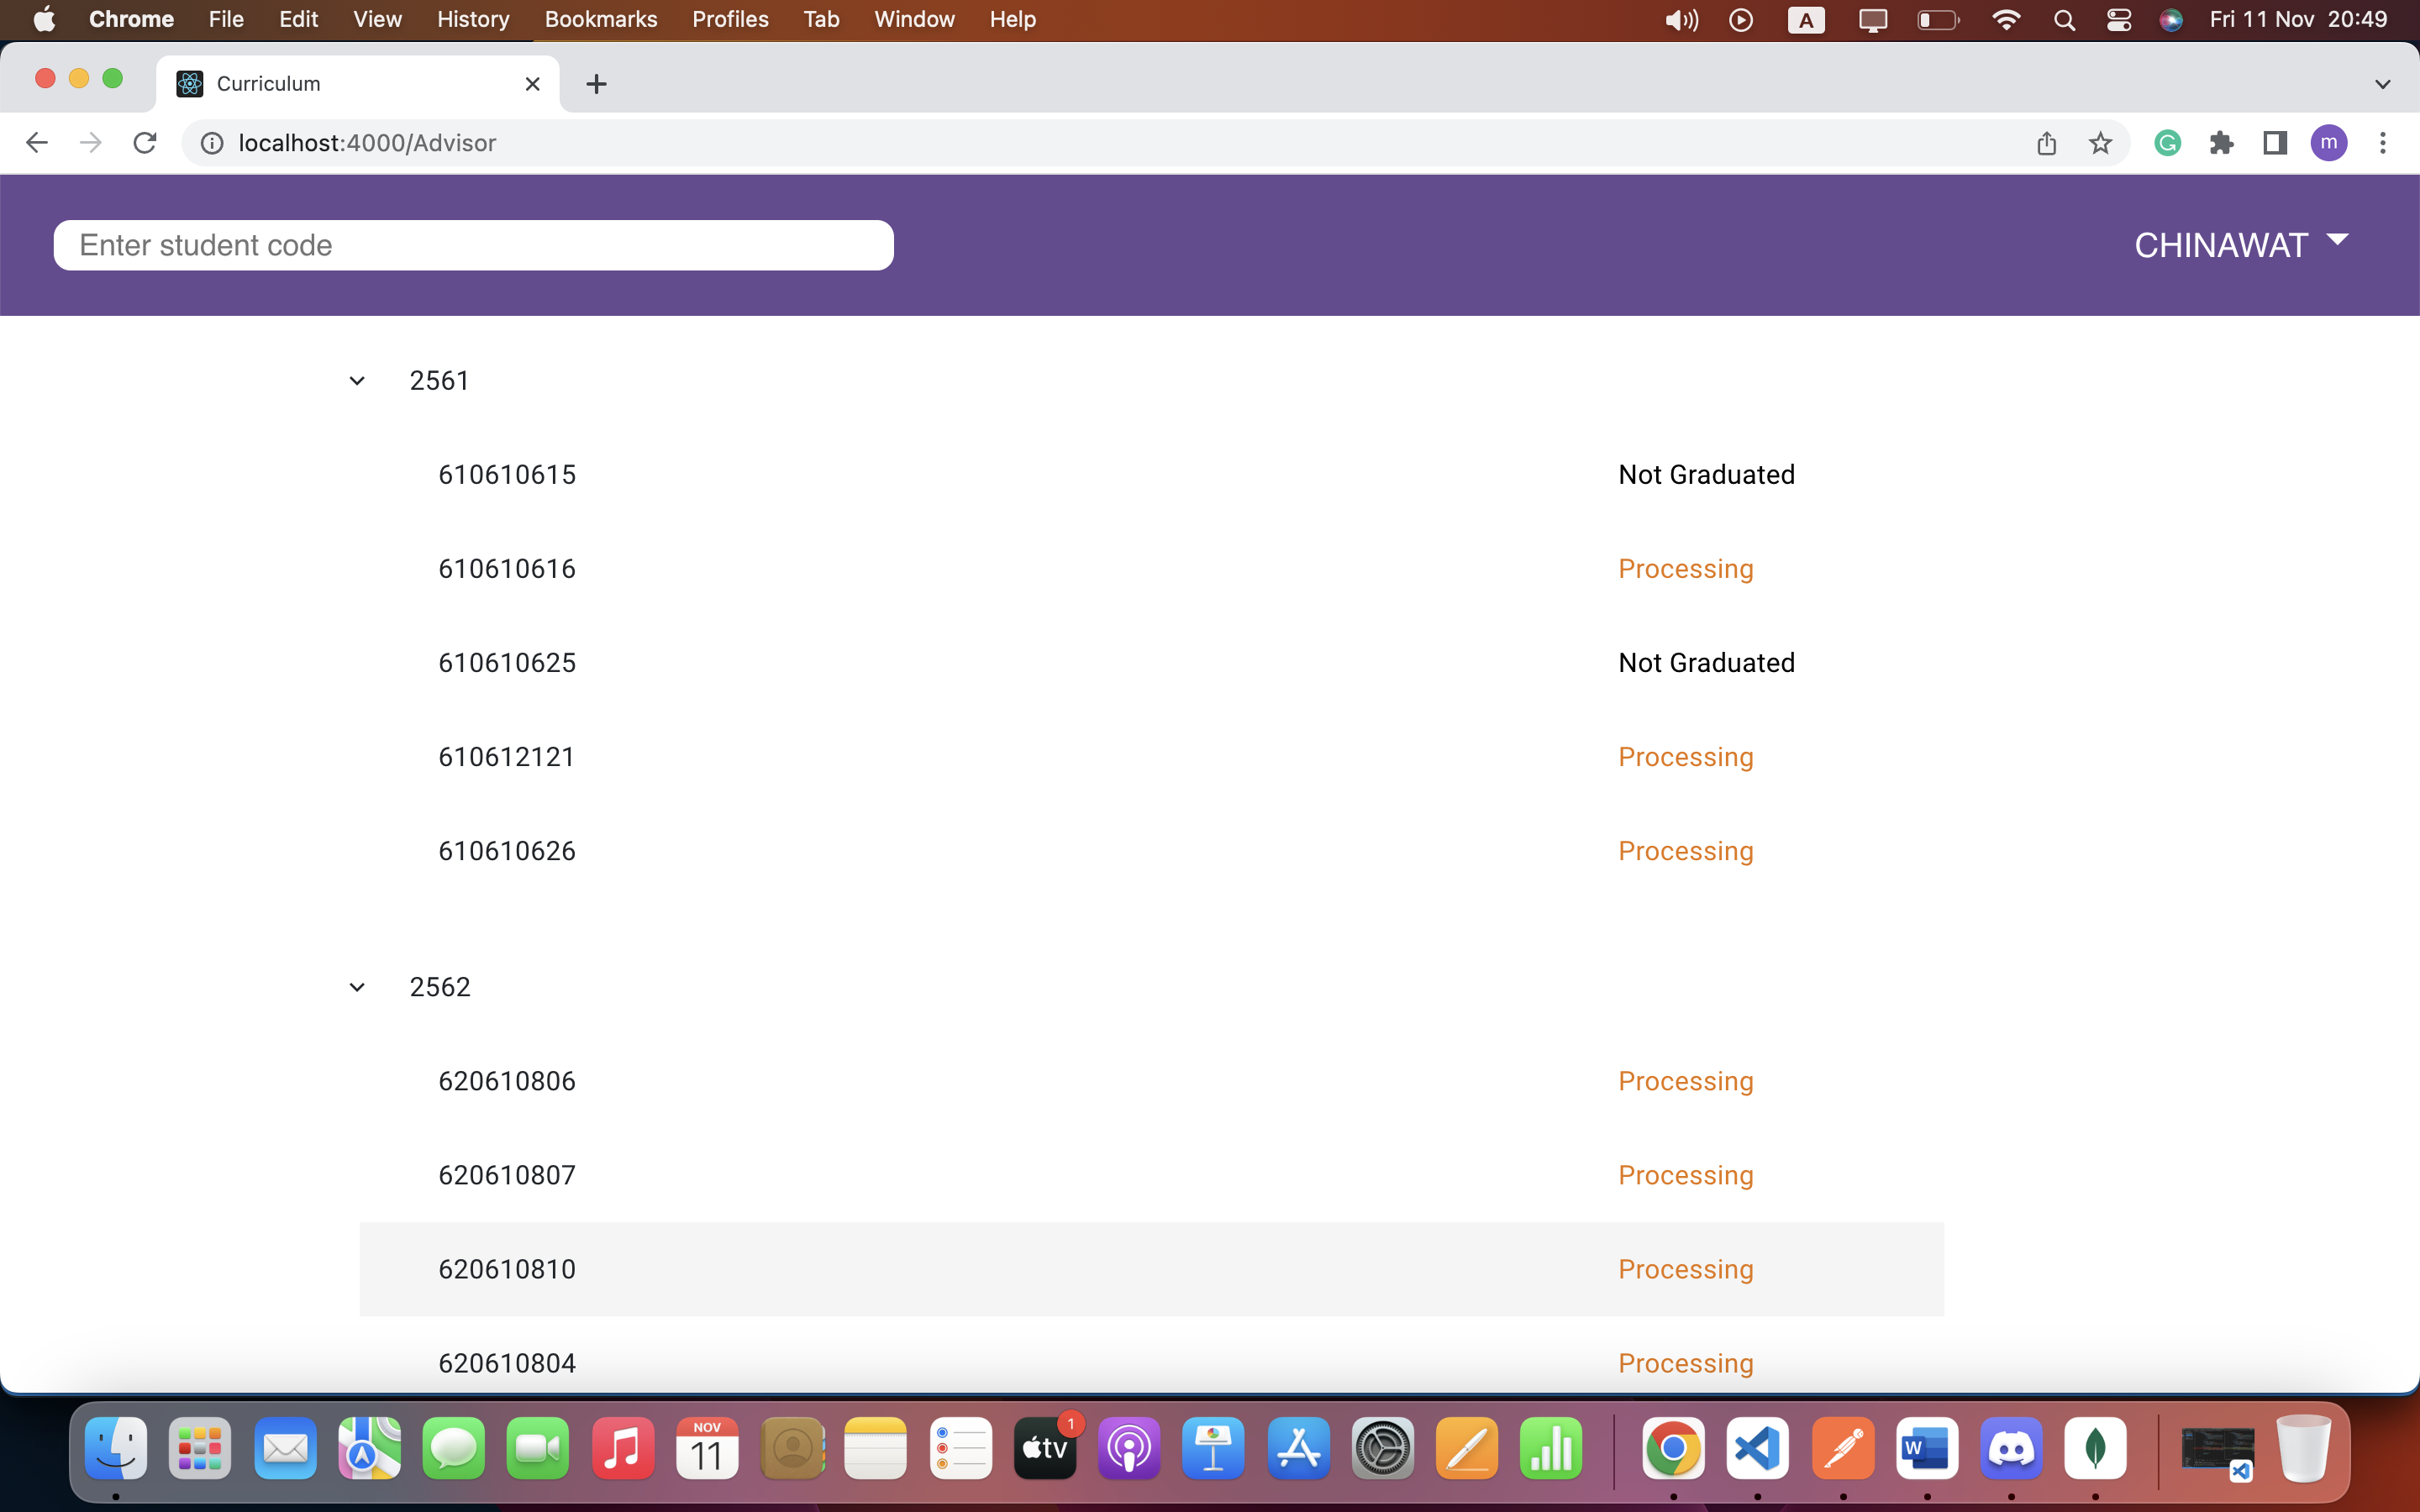
\includegraphics[width=0.8\textwidth]{advisor.png}
    \caption{หน้าเเสดงสถานะนักศึกษา ของอาจารย์ที่ปรึกษา}
    \label{fig:advisor}
  \end{center}
\end{figure}

การใช้งานของอาจารย์ที่ปรึกษา ระบบจะแบ่งกลุ่มของนักศึกษาที่อยู่ในการดูแลตามปีการศึกษาที่นักศึกษาเข้าศึกษา ซึ่ง
อาจารย์ที่ปรึกษาสามารถเข้าไปดูความคืบหน้าของนักศึกษาได้จาก สถานะทางริมขวามือของรหัสนักศึกษา

\subsection{หน้าเว็บสำหรับผู้ดูแลหลักสูตร}

\begin{figure}[H]
  \begin{center}
    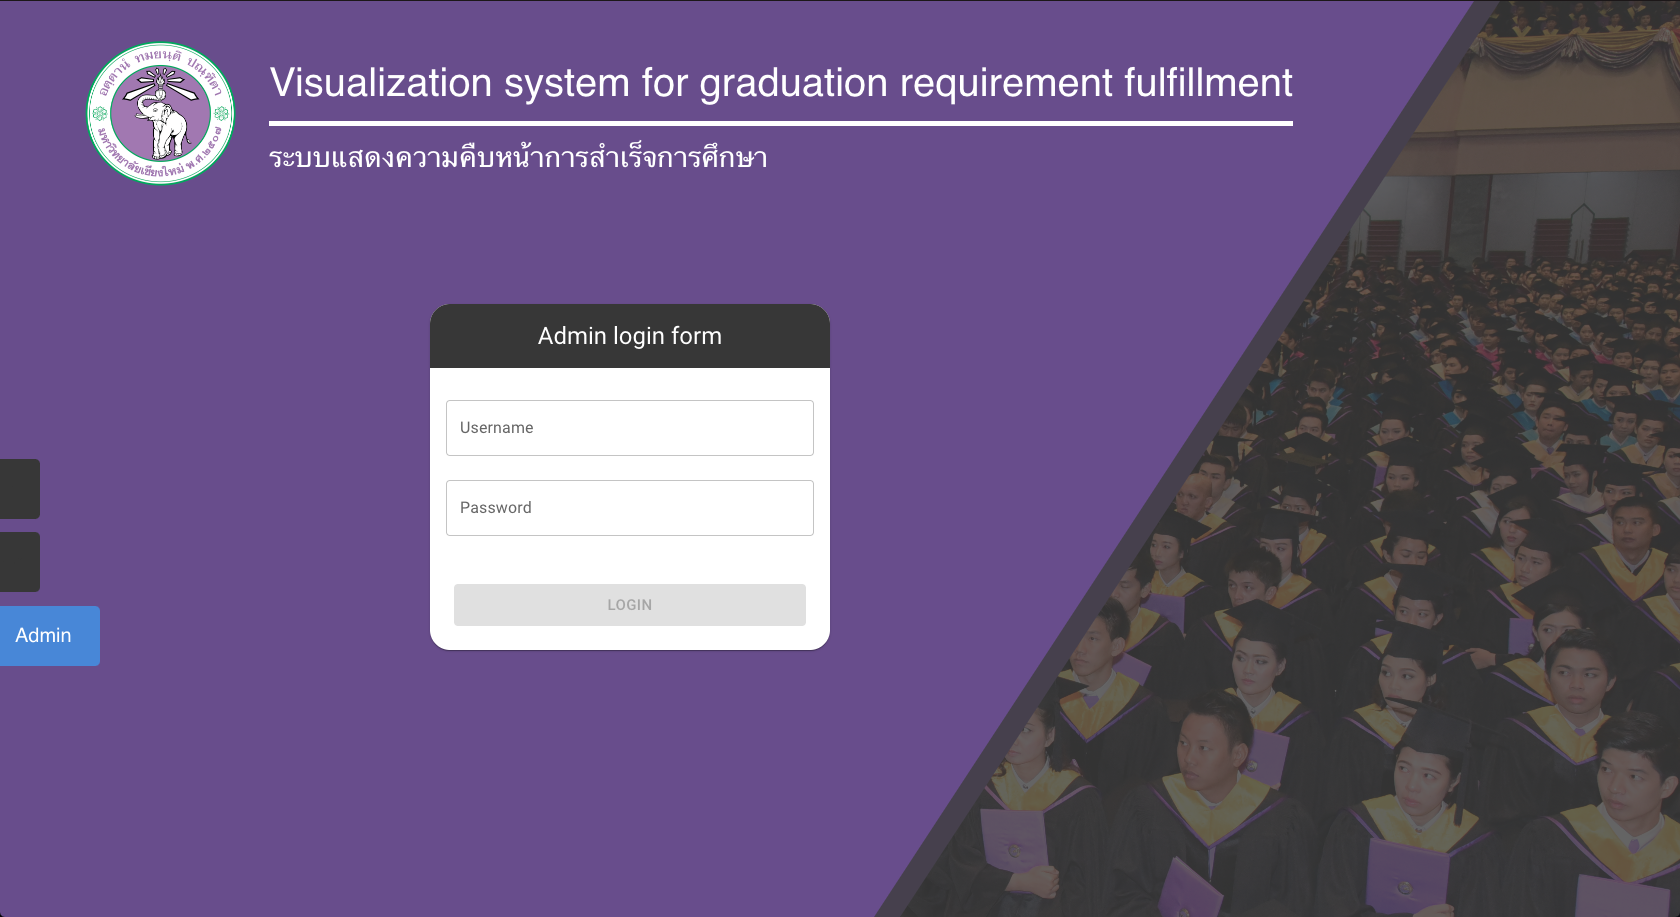
\includegraphics[width=0.8\textwidth]{admin_login.png}
    \caption{หน้า Admin Login}
    \label{fig:admin_login}
  \end{center}
\end{figure}

\begin{figure}[H]
  \begin{center}
    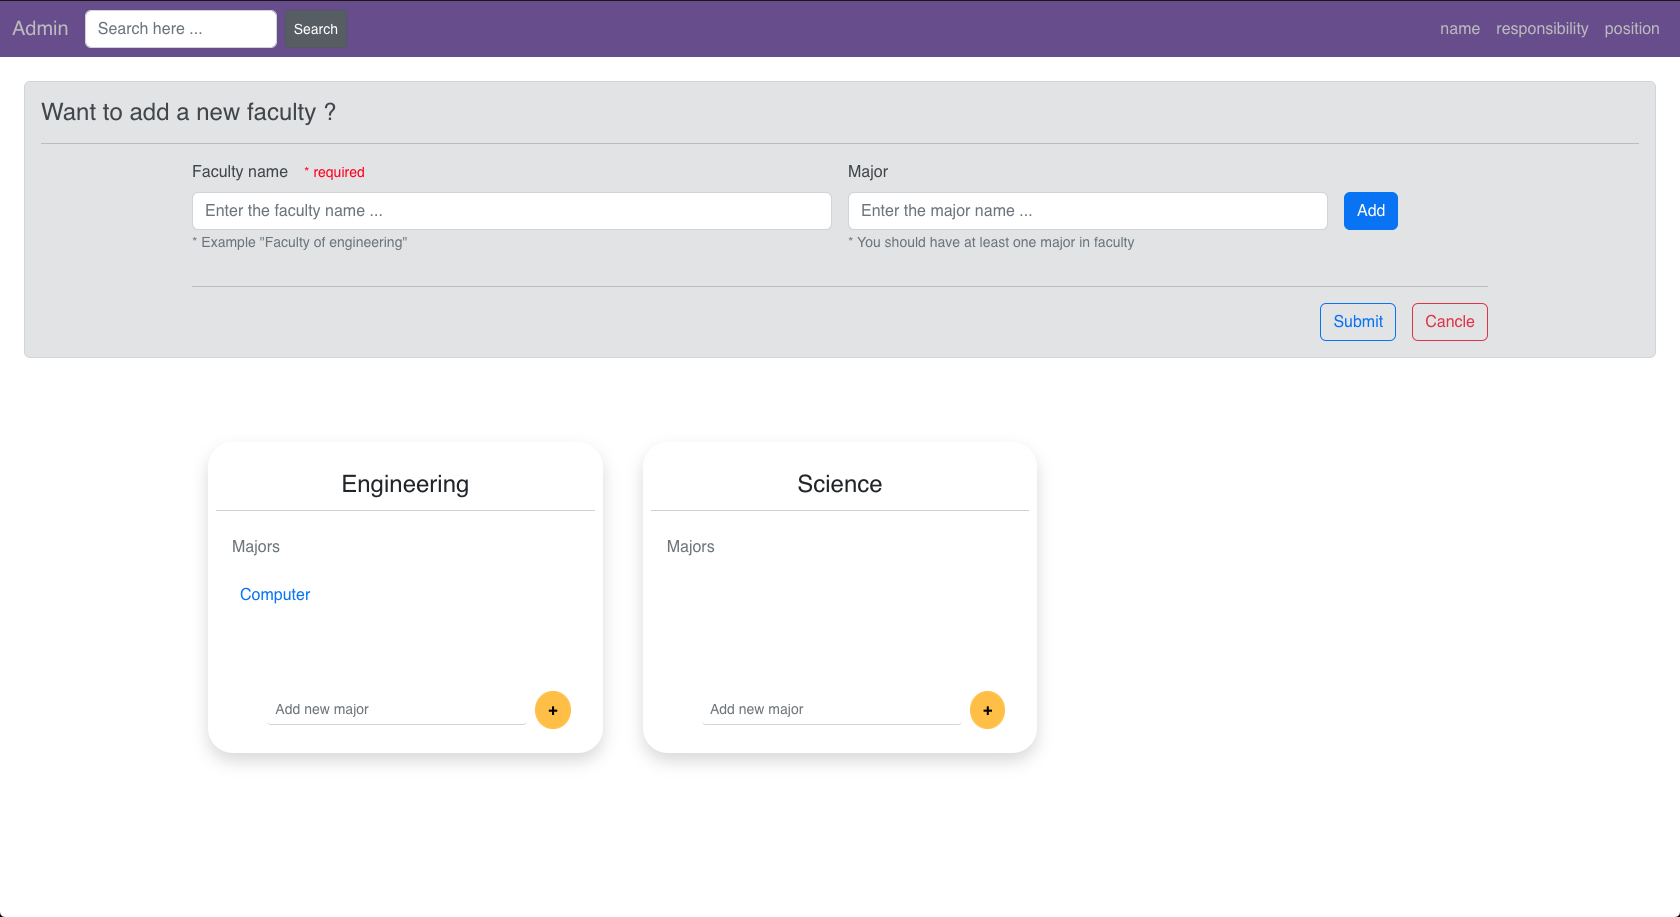
\includegraphics[width=0.8\textwidth]{big_admin.png}
    \caption{หน้าจัดการข้อมูลในระดับ คณะ และสาขา}
    \label{fig:big_admin}
  \end{center}
\end{figure}

\begin{figure}[H]
  \begin{center}
    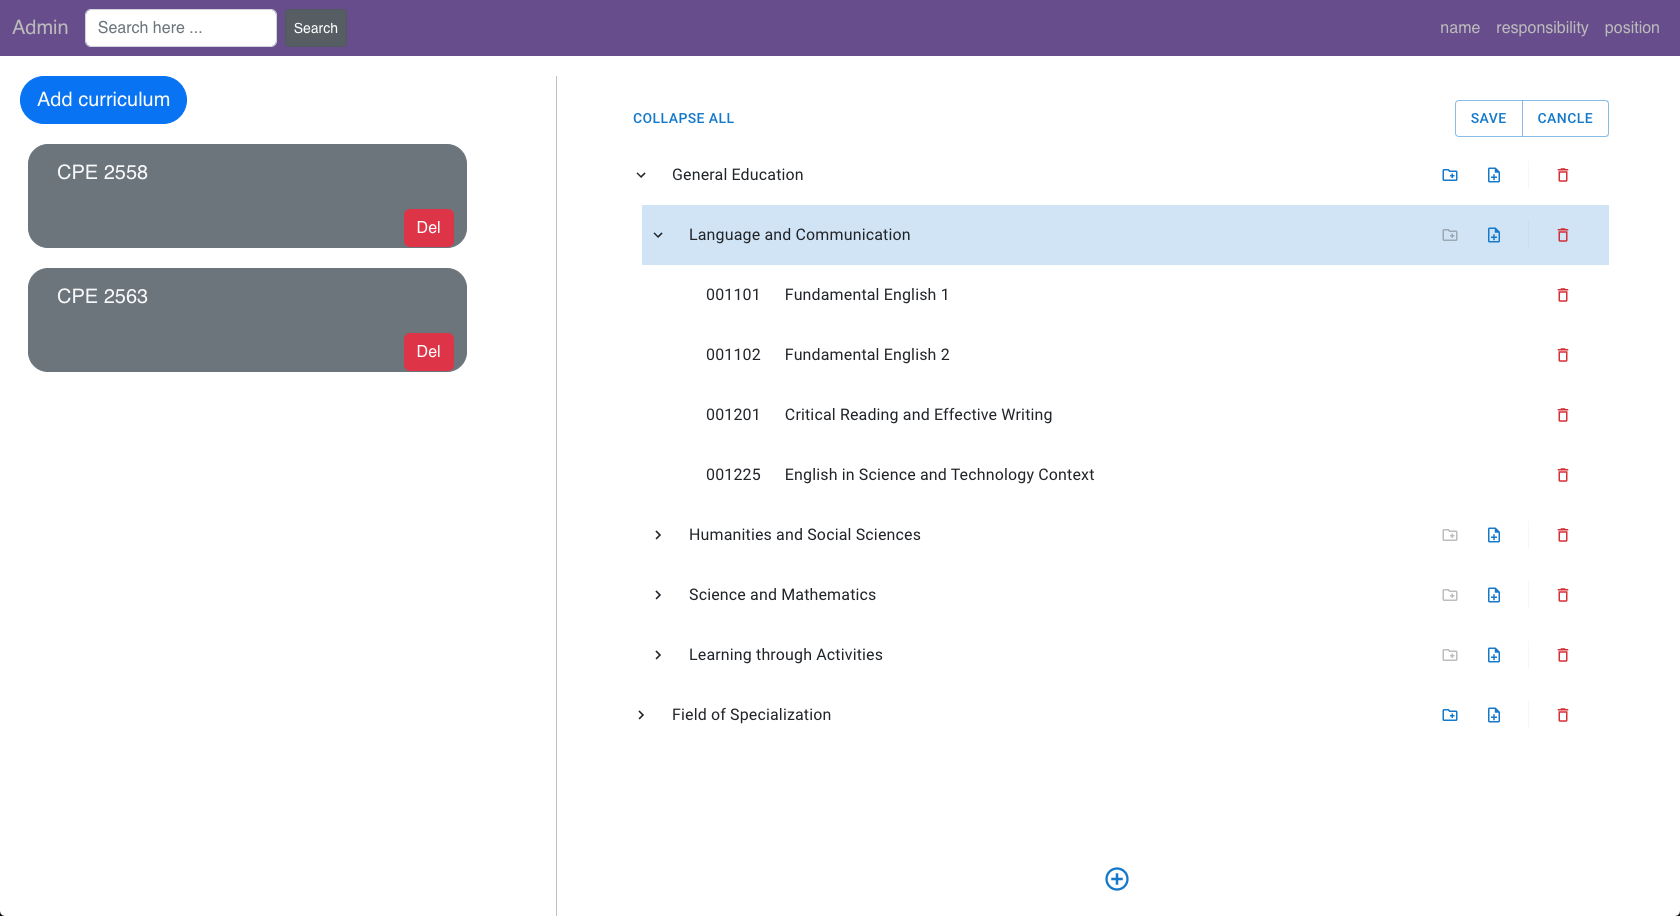
\includegraphics[width=0.8\textwidth]{admin.png}
    \caption{หน้าจัดการข้อมูลในระดับหลักสูตร}
    \label{fig:admin}
  \end{center}
\end{figure}

การใช้งานของผู้ดูแลระบบหรือแอดมิน ในส่วนของแอดมินในขณะนี้จะแบ่งออกเป็น 3 แบบตามความสามารถในการจัดการ
หลักสูตร ได้แก่ 1. แอดมินระดับมหาวิทยาลัย จะสามารถจัดการหลักสูตรได้ทุกหลักสูตรในมหาวิทยาลัย ซึ่งจะสามารถจัดการ(CUD
(create , update and delete))ได้ตั้งแต่ระดับคณะ สาขาวิชา และหลักสูตรในแต่ละปี รวมถึงการแก้ไข เพิ่ม และลบรายวิชาใน
หลักสูตรนั้นๆด้วย 2. แอดมินระดับคณะสามารถจัดการหลักสูตรได้เพียงแค่ในคณะที่ตนเองดูแลอยู่เท่านั้น ซึ่งจะ CUD ได้ตั้งแต่ระดับ
สาขาวิชาและหลักสูตรในแต่ละปี รวมถึงการแก้ไข เพิ่ม และลบรายวิชาในหลักสูตรนั้นๆด้วย 3. แอดมินระดับภาควิชาสามารถจัดการ
หลักสูตรได้ภายในภาควิชาที่ตนเองดูแลเท่านั้น ซึ่งจะ CUD ได้ในระดับหลักสูตรในแต่ละปี รวมถึงการแก้ไข เพิ่ม และลบรายวิชาใน
หลักสูตรนั้นๆด้วย

\subsection{สรุปข้อมูลการศึกษาหลักสูตร}

\begin{center}
  จากการศีกษาหลักสูตรระดับปริญญาตรีทุกสาขาวิชาของทุกคณะในมหาวิทยาลัยเชียงใหม่ จํานวน 185 หลักสูตร ซึ่งได้ทําการจําแนกความซับซ้อนของแต่ละหลักสูตรเป็นหนึ่งใน 4 ระดับ ดังต่อไปนี้
\end{center}

\begin{figure}[H]
  \begin{center}
    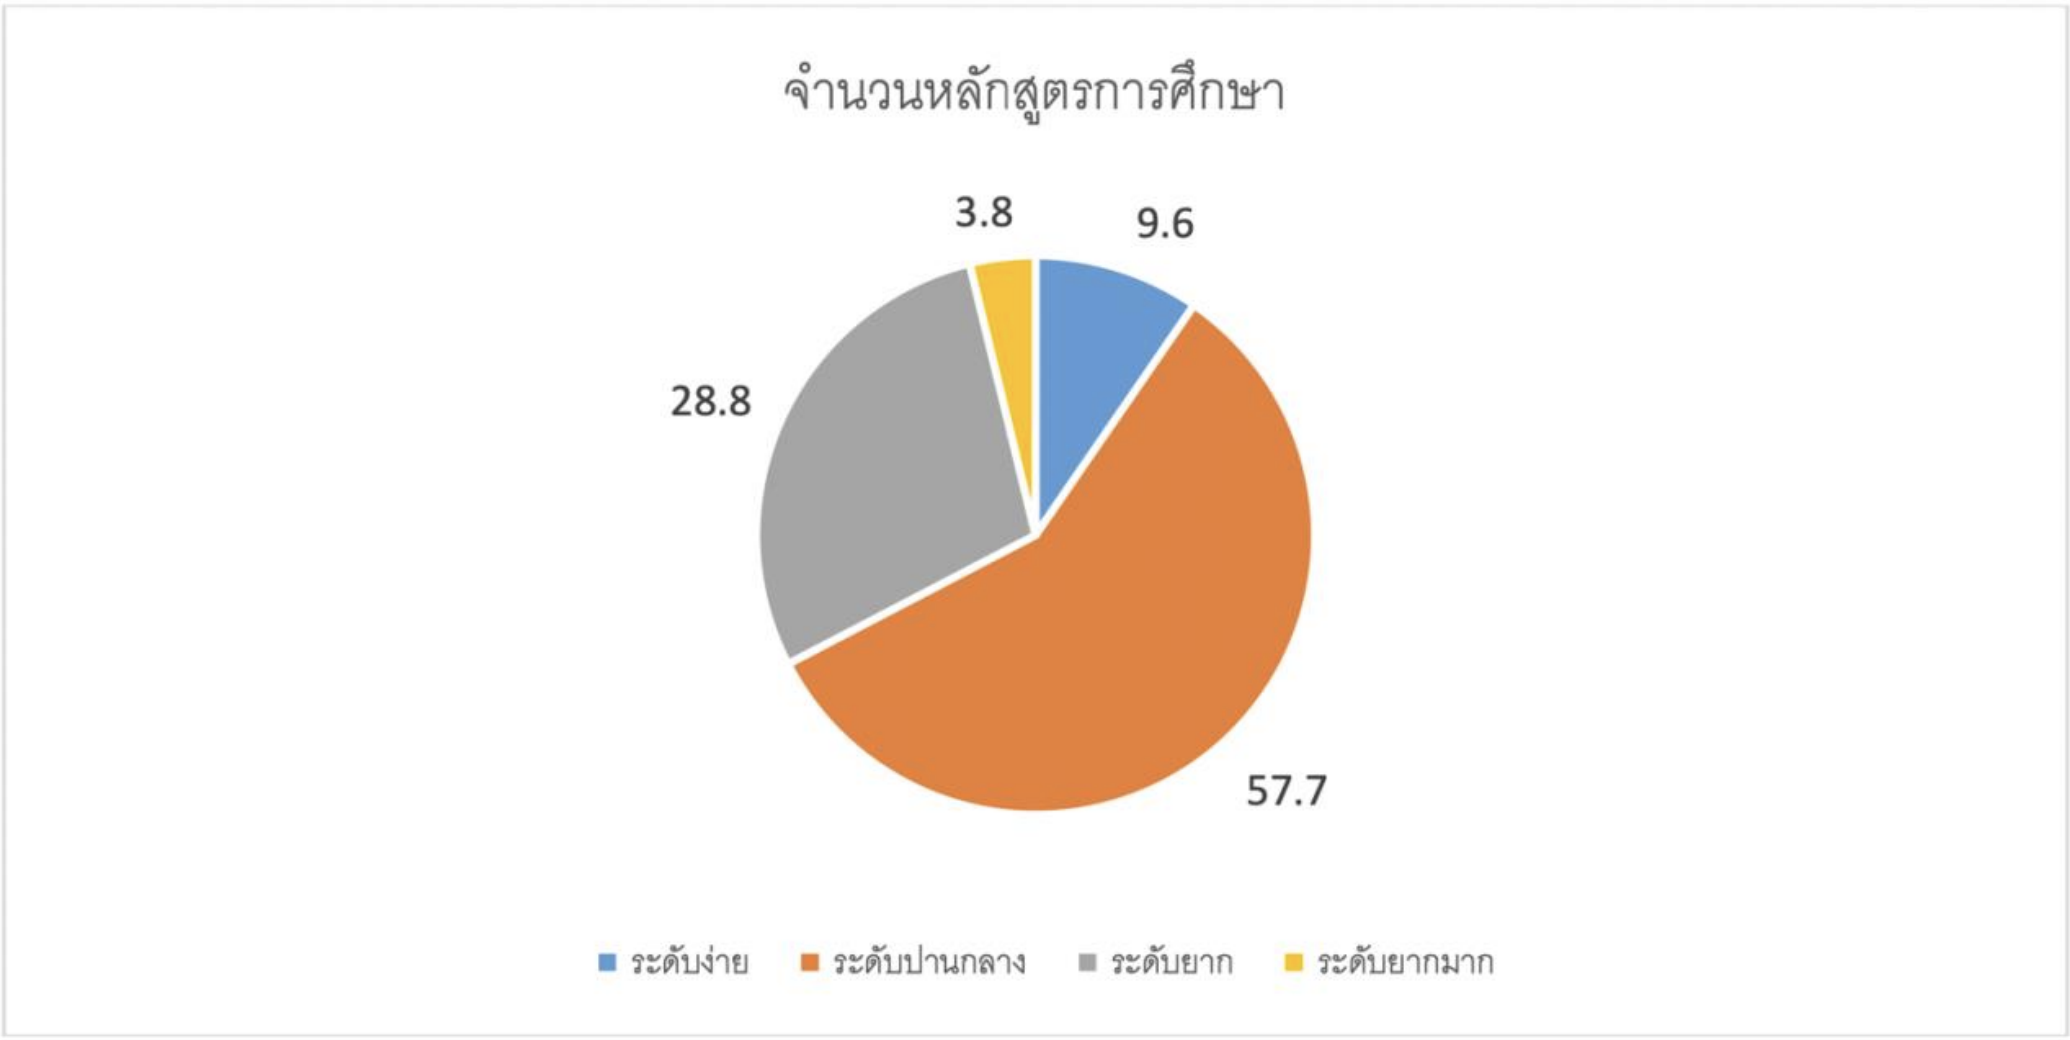
\includegraphics[width=0.8\textwidth]{chart.png}
    \caption{สรุปภาพการศึกษาหลักสูตร}
    \label{fig:chart}
  \end{center}
\end{figure}

\begin{center}
  \begin{minipage}[c]{0.5\linewidth}
     \begin{itemize}
       \item ระดับง่าย 9.6 \%
       \item ระดับปานกลาง 57.7 \%
       \item ระดับยาก 28.8 \%
       \item ระดับยากมาก 3.8 \%
     \end{itemize}
  \end{minipage}
\end{center}

เห็นได้ว่าในหลักสูตรที่พบเห็นได้บ่อยนั้นจะถูกจัดอยู่ในหลักสูตรระดับปานกลาง ดังนั้นในช่วงแรกของการ พัฒนา ผู้พัฒนาจะเริ่มจาก
หลักสูตรระดับปานกลางก่อน และหลักสูตรในระดับยากมากมีทั้งหมด 7 หลักสูตรมีค่าเปอร์เซ็นต์อยู่ที่ 3.8 \% ซึ่งจะมีเพียงบาง
สาขาวิชาเท่านั้น ดังนั้นหลักสูตรที่ถูกจัดอยู่ในระดับ ยากมากทั้งหมดทางผู้พัฒนาจึงขอละเว้นไว้จากขอบเขตของโครงงานนี้


\subsection{การออกแบบโครงสร้างพื้นฐานของข้อมูล}

จากการศึกษาหลักสูตรระดับปริญญาตรีทุกสาขาวิชาของทุกคณะในมหาวิทยาลัยเชียงใหม่ ทําให้เข้าใจโครงสร้าง
เเละรูปเเบบต่างๆของหลักสูตรจึงสามารถสรุป General data model ขึ้นมาได้ ที่จะถูกนําไปใช้สร้าง database ต่อไป

\begin{figure}[H]
  \begin{center}
    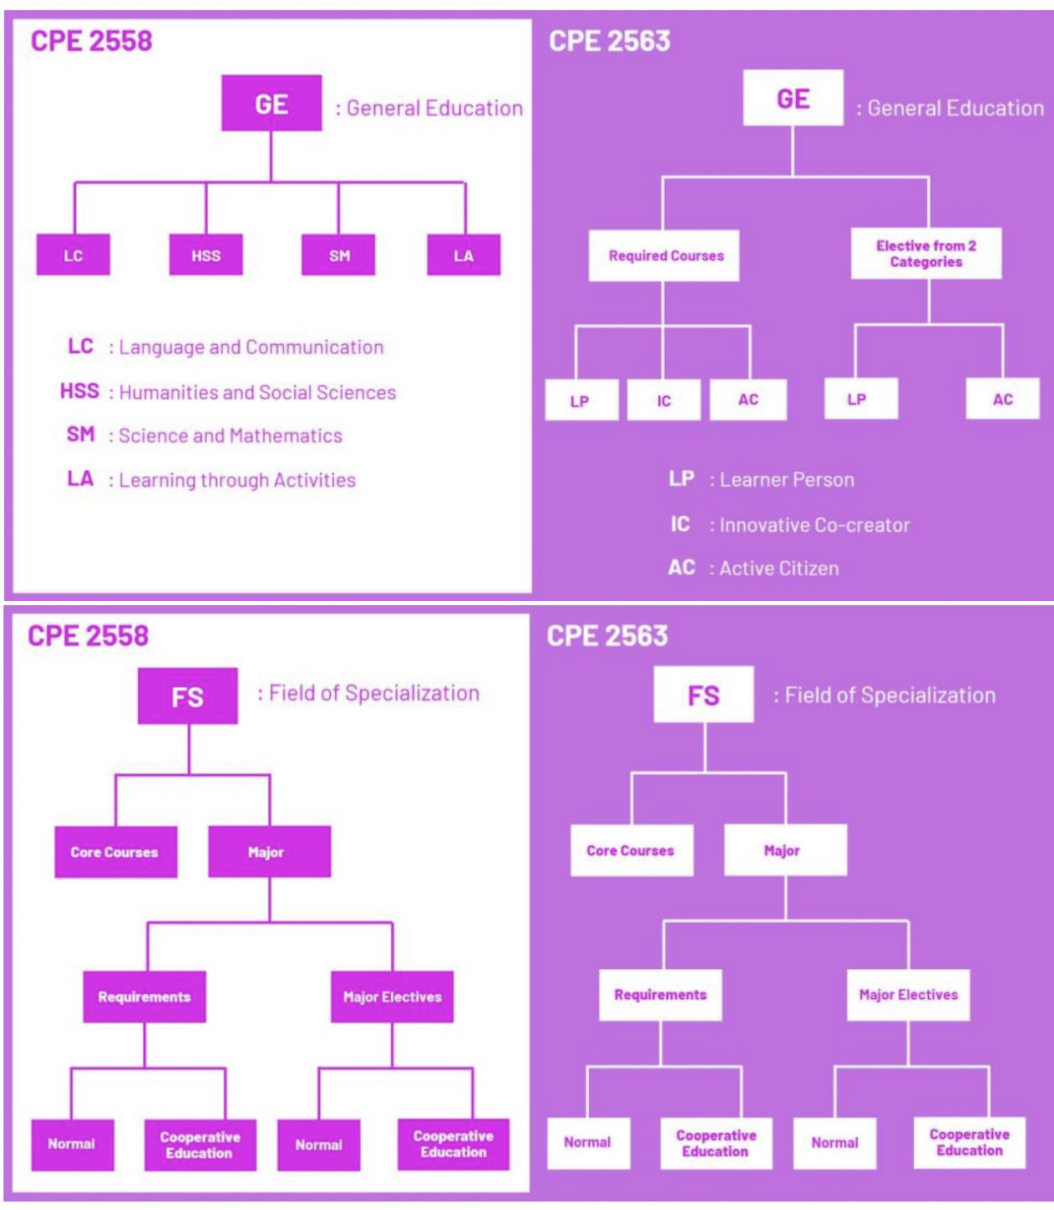
\includegraphics[width=0.8\textwidth]{dModel.png}
    \caption{ตัวอย่าง Data model ของหลักสูตรวิศวกรรมคอมพิวเตอร์}
    \label{fig:dModel}
  \end{center}
\end{figure}

จาก Data model จะสังเกตุได้ว่า ทั้ง 2 หลักสูตรจะมี FS ที่เหมือนกันทำให้สามารถทำ Curriculum data sharing ได้ซึ่ง
ยังมีหลักสูตรอีกจำนวนมาก ที่สามารถทำ Curriculum data sharing ได้

\begin{figure}[H]
  \begin{center}
    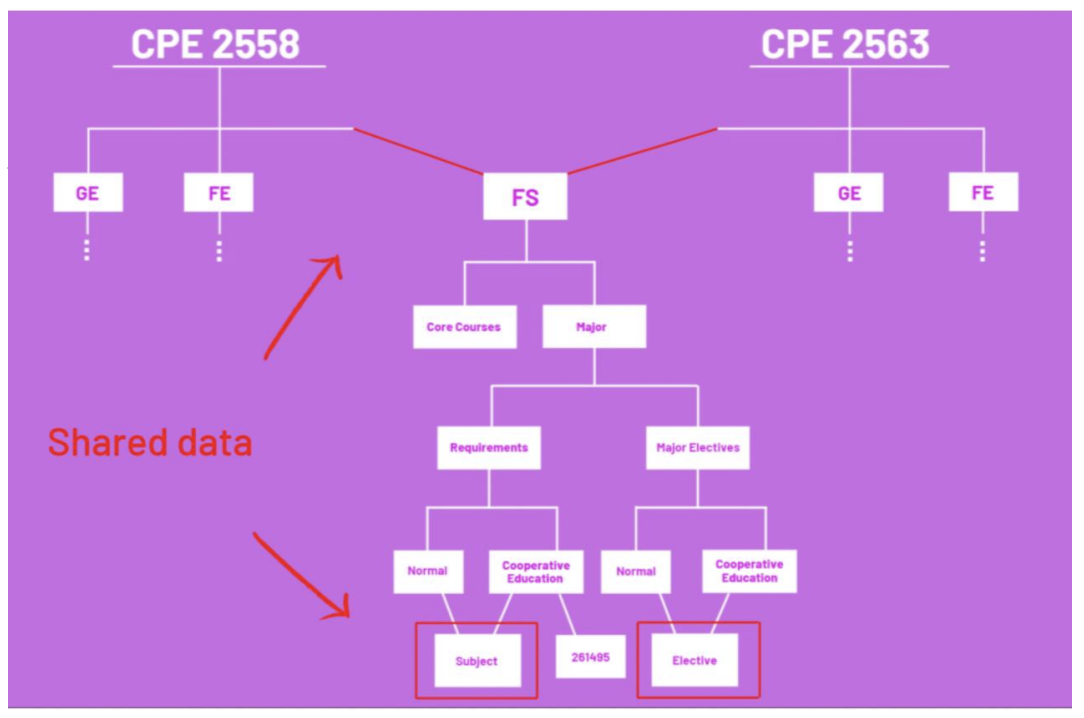
\includegraphics[width=0.8\textwidth]{model.png}
    \caption{Data Sharing}
    \label{fig:model}
  \end{center}
\end{figure}

\begin{enumerate}
  \item Curriculum data sharing ในกรณีนี้เป็นการ share FS ของหลักสูตร 2558 และ 2563
  \item Node data sharing ใน FS ที่ทั้ง 2 หลักสูตรใช้ร่วมกัน มีการ share Subject และ Elective ระหว่าง Normal และ
  Cooperative Education
\end{enumerate}

\section{ขั้นตอนการดำเนินงาน}
\subsection{ศึกษาโครงสร้างหลักสูตร}
จากขอบเขตของโครงงานที่ตั้งเป้าหมายให้เว็ปแอปพลิเคชั่นนั้นสามารถรองรับได้ในทุกหลักสูตรจึงเป็นผลให้ต้องศึกษาโครงสร้างหลักสูตรในแต่ละหลักสูตร 
และหลังจากที่ทําการศึกษาแล้วนั้นพบว่าในปัจจุบันจะมีหลักสูตรที่ใช้กันอย่างมากในมหาวิทยาลัยเชียงใหม่นั่นก็คือหลักสูตรปีการศึกษา 2558 และหลักสูตรปีการศึกษา 2563 (1 หลักสูตรสามารถใช้ได้ 5 ปีการศึกษา) 
แต่ยังคงมีหลักสูตรในบางสาขาวิชาที่มีการปรับปรุงหลักสูตรก่อนครบ 5 ปีการศึกษา จึงเป็นผลให้ต้องศึกษาโครงสร้างของหลักสูตรนั้นอย่างละเอียดอีกครั้งเพื่อตรวจสอบดูว่ามีหลักสูตรใดบ้างที่มีการปรับปรุงหลักสูตรก่อนครบ 5 ปีการศึกษา 
เพราะถ้าหากพบว่าหลักสูตรใดมีการปรับปรุงหลักสูตรก่อนครบ 5 ปีการศึกษา ทางผู้พัฒนาจะนับเป็นหลักสูตรใหม่ตามปีการศึกษาที่ประกาศใช้หลักสูตรนั้นทันที
\subsection{จำแนกระดับความซับซ้อนของหลักสูตร}
ในระหว่างที่ทำการศึกษาโครงสร้างหลักสูตรแต่ละอันนั้นผู้พัฒนาได้ทำการจำแนกหลักสูตรตามระดับความซับซ้อนของหลักสูตรด้วยเช่นกัน 
โดยทำการจำแนกจากความสามารถในการเลือกแผนการเรียนภายในหลักสูตรนั้นๆซึ่งจะได้ออกมาดังนี้
\begin{enumerate}
  \item หลักสูตรระดับง่าย - คือหลักสูตรที่ไม่สามารถเลือกแผนการเรียนตามความสนใจของนักศึกษาได้ กล่าวอีกนัยนึงคือมีแค่แผนการเรียนเดียวในหลักสูตรนั้นจึงทำให้มีโครงสร้างหลักสูตรที่ไม่ซับซ้อน
	ตัวอย่างเช่น
  \begin{itemize}
    \item หลักสูตรปีการศึกษา 2564 สาขาวิศวกรรมหุ่นยนต์ ที่มีแผนการเรียนแบบปกติ ( Normal ) เพียงอย่างเดียว
    \item หลักสูตรปีการศึกษา 2561 สาขาพยาบาลศาสตร์ ที่มีแผนการเรียนแบบสหกิจศึกษา ( Co-operative ) เพียงอย่างเดียว
  \end{itemize}
  \item หลักสูตรระดับปานกลาง - คือหลักสูตรที่มีแผนการเรียนทั้งแบบปกติและแบบสหกิจศึกษา ทำให้สามารถเลือกเรียนได้มากกว่า 1 รูปแบบ ดังนั้นโครงสร้างหลักสูตรจึงมีความซับซ้อนมากขึ้น ซึ่งหลักสูตรในระดับปานกลางนี้จะพบได้ในหลายคณะ
  ตัวอย่างเช่น
  \begin{itemize}
    \item หลักสูตรปีการศึกษา 2558 และ 2563 สาขาวิศวกรรมคอมพิวเตอร์
  \end{itemize}
  \item หลักสูตรระดับยาก - คือหลักสูตรที่มีแผนการเรียนทั้งแบบปกติ แบบสหกิจศึกษา และยังสามารถเลือกความถนัดในหลักสูตรของตนเองได้อย่างอิสระ ทำให้โครงสร้างหลักสูตรนั้นมีความซับซ้อนมาก และต้องทำการเทียบกระบวนวิชาที่สอดคล้องกันในแต่ละหมวดของความถนัด
  ตัวอย่างเช่น
  \begin{itemize}
    \item หลักสูตรปีการศึกษา 2558 และ 2563 สาขาวิศวกรรมไฟฟ้า ที่สามารถเลือกแผนการเรียนได้ 2 รูปแบบและสามารถเลือกหมวดความถนัดภายในสาขาวิชาตามที่สนใจได้อีก 2 หมวดได้แก่ ไฟฟ้ากำลัง และไฟฟ้าสื่อสาร
  \end{itemize}
  \item หลักสูตรระดับยากมาก - คือหลักสูตรที่มีแผนการเรียนทั้งแบบปกติ แบบสหกิจศึกษา เลือกหมวดความถนัด และในหมวดความถนัดแต่ละอันก็ยังคงเลือกได้อีกว่าจะเรียนหมวดความถนัดย่อยใดต่อไป ทำให้โครงสร้างหลักสูตรนั้นมีความซับซ้อนอยู่ในระดับยากที่สุด
  ตัวอย่างเช่น
  \begin{itemize}
    \item หลักสูตรปีการศึกษา 2558 และ 2563 คณะเภสัชศาสตร์
    \item หลักสูตรปีการศึกษา 2558 และ 2563 คณะเกษตรศาสตร์ สาชาวิชาเกษตรศาสตร์
  \end{itemize}
\end{enumerate}

\subsection{ออกแบบระบบ}
\begin{itemize}
  \item ออกแบบ UX/UI ของระบบด้วยโปรแกรม Adobe XD แต่เนื่องจากเกิดปัญหาในการใช้ plug-in ของโปรแกรม Adobe XD ผู้พัฒนาจึงเปลี่ยนไปใช้โปรแกรม 
  Figma แทน
  \item ออกเเบบ Data Model เเละ Database
\end{itemize}

\subsection{พัฒนาระบบ}

Frontend
\begin{itemize}
  \item พัฒนาหน้าเว็บไซค์ตามที่ได้ออกแบบ UX/UI เอาไว้ โดยนำข้อมูลจำลองที่ออกแบบมาใช้เป็นตัวอย่างในการพัฒนาขั้นต้น
  \item เชื่อมต่อ Apollo client ในฝั่ง front-end
  \item พัฒนาและเรียกใช้งาน query ต่างๆเพื่อดึงข้อมูลจริงจากฝั่ง back-end
\end{itemize}
Backend
\begin{itemize}
  \item คํานวณ เทียบหลักสูตรการศึกษาที่มีในระบบ กับข้อมูลการลงทะเบียนของนักศึกษา เพื่อเช็คสถานะต่างๆ 
  ของนักศึกษา อาทิ (เกรด, เกรดเฉลี่ย, รายวิชาที่ลง, หมวดต่างๆที่ต้องลงตามหลักสูตร ) เเละส่งออกมาเป็น ข้อมูลที่มีลําดับขั้น(Tree) ก่อนส่งต่อให้ Frontend
  \item พัฒนา Backend server ประมวลผลข้อมูลก่อนสร้างก้อนข้อมูล ด้วย Graphql 
  \item พัฒนา Graphql schema และ Graphql resolvers เพื่อตอบสนองการดึงข้อมูลผ่าน Frontend ด้วย Apollo client
  \item พัฒนา Apollo server ในฝั่ง back-end
  \item พัฒนาเเละ จัดการ ฐานข้อมูล MongoDB ผ่าน Mongoose
\end{itemize}

\subsection{ทดลองใช้งาน}
\begin{itemize}
  \item ผู้พัฒนาได้ทดลองล็อกอินผ่าน CMU Account เพื่อเข้าใช้งานระบบและพัฒนาระบบอยู่เสมอ
  \item ให้นักศึกษา CPE ทดลองเข้าสู่ระบบโดยล็อกอินผ่านคอมพิวเตอร์ของผู้พัฒนา (เวอร์ชันก่อน deploy และ test)
  \item Deploy ระบบให้สามารถเข้าใช้งานผ่านลิงก์ พร้อมทั้งแนบแบบสอบถามเพื่อเก็บผลประเมินหลังการใช้งานระบบแสดงความคืบหน้าการสำเร็จการศึกษา
\end{itemize}

